% Options for packages loaded elsewhere
\PassOptionsToPackage{unicode=true}{hyperref}
\PassOptionsToPackage{hyphens}{url}
%
\documentclass[
]{book}
\usepackage{lmodern}
\usepackage{amssymb,amsmath}
\usepackage{ifxetex,ifluatex}
\ifnum 0\ifxetex 1\fi\ifluatex 1\fi=0 % if pdftex
  \usepackage[T1]{fontenc}
  \usepackage[utf8]{inputenc}
  \usepackage{textcomp} % provides euro and other symbols
\else % if luatex or xelatex
  \usepackage{unicode-math}
  \defaultfontfeatures{Scale=MatchLowercase}
  \defaultfontfeatures[\rmfamily]{Ligatures=TeX,Scale=1}
\fi
% Use upquote if available, for straight quotes in verbatim environments
\IfFileExists{upquote.sty}{\usepackage{upquote}}{}
\IfFileExists{microtype.sty}{% use microtype if available
  \usepackage[]{microtype}
  \UseMicrotypeSet[protrusion]{basicmath} % disable protrusion for tt fonts
}{}
\makeatletter
\@ifundefined{KOMAClassName}{% if non-KOMA class
  \IfFileExists{parskip.sty}{%
    \usepackage{parskip}
  }{% else
    \setlength{\parindent}{0pt}
    \setlength{\parskip}{6pt plus 2pt minus 1pt}}
}{% if KOMA class
  \KOMAoptions{parskip=half}}
\makeatother
\usepackage{xcolor}
\IfFileExists{xurl.sty}{\usepackage{xurl}}{} % add URL line breaks if available
\IfFileExists{bookmark.sty}{\usepackage{bookmark}}{\usepackage{hyperref}}
\hypersetup{
  pdftitle={A Minimal Book Example},
  pdfauthor={Yihui Xie},
  hidelinks,
}
\urlstyle{same} % disable monospaced font for URLs
\usepackage{color}
\usepackage{fancyvrb}
\newcommand{\VerbBar}{|}
\newcommand{\VERB}{\Verb[commandchars=\\\{\}]}
\DefineVerbatimEnvironment{Highlighting}{Verbatim}{commandchars=\\\{\}}
% Add ',fontsize=\small' for more characters per line
\usepackage{framed}
\definecolor{shadecolor}{RGB}{248,248,248}
\newenvironment{Shaded}{\begin{snugshade}}{\end{snugshade}}
\newcommand{\AlertTok}[1]{\textcolor[rgb]{0.94,0.16,0.16}{#1}}
\newcommand{\AnnotationTok}[1]{\textcolor[rgb]{0.56,0.35,0.01}{\textbf{\textit{#1}}}}
\newcommand{\AttributeTok}[1]{\textcolor[rgb]{0.77,0.63,0.00}{#1}}
\newcommand{\BaseNTok}[1]{\textcolor[rgb]{0.00,0.00,0.81}{#1}}
\newcommand{\BuiltInTok}[1]{#1}
\newcommand{\CharTok}[1]{\textcolor[rgb]{0.31,0.60,0.02}{#1}}
\newcommand{\CommentTok}[1]{\textcolor[rgb]{0.56,0.35,0.01}{\textit{#1}}}
\newcommand{\CommentVarTok}[1]{\textcolor[rgb]{0.56,0.35,0.01}{\textbf{\textit{#1}}}}
\newcommand{\ConstantTok}[1]{\textcolor[rgb]{0.00,0.00,0.00}{#1}}
\newcommand{\ControlFlowTok}[1]{\textcolor[rgb]{0.13,0.29,0.53}{\textbf{#1}}}
\newcommand{\DataTypeTok}[1]{\textcolor[rgb]{0.13,0.29,0.53}{#1}}
\newcommand{\DecValTok}[1]{\textcolor[rgb]{0.00,0.00,0.81}{#1}}
\newcommand{\DocumentationTok}[1]{\textcolor[rgb]{0.56,0.35,0.01}{\textbf{\textit{#1}}}}
\newcommand{\ErrorTok}[1]{\textcolor[rgb]{0.64,0.00,0.00}{\textbf{#1}}}
\newcommand{\ExtensionTok}[1]{#1}
\newcommand{\FloatTok}[1]{\textcolor[rgb]{0.00,0.00,0.81}{#1}}
\newcommand{\FunctionTok}[1]{\textcolor[rgb]{0.00,0.00,0.00}{#1}}
\newcommand{\ImportTok}[1]{#1}
\newcommand{\InformationTok}[1]{\textcolor[rgb]{0.56,0.35,0.01}{\textbf{\textit{#1}}}}
\newcommand{\KeywordTok}[1]{\textcolor[rgb]{0.13,0.29,0.53}{\textbf{#1}}}
\newcommand{\NormalTok}[1]{#1}
\newcommand{\OperatorTok}[1]{\textcolor[rgb]{0.81,0.36,0.00}{\textbf{#1}}}
\newcommand{\OtherTok}[1]{\textcolor[rgb]{0.56,0.35,0.01}{#1}}
\newcommand{\PreprocessorTok}[1]{\textcolor[rgb]{0.56,0.35,0.01}{\textit{#1}}}
\newcommand{\RegionMarkerTok}[1]{#1}
\newcommand{\SpecialCharTok}[1]{\textcolor[rgb]{0.00,0.00,0.00}{#1}}
\newcommand{\SpecialStringTok}[1]{\textcolor[rgb]{0.31,0.60,0.02}{#1}}
\newcommand{\StringTok}[1]{\textcolor[rgb]{0.31,0.60,0.02}{#1}}
\newcommand{\VariableTok}[1]{\textcolor[rgb]{0.00,0.00,0.00}{#1}}
\newcommand{\VerbatimStringTok}[1]{\textcolor[rgb]{0.31,0.60,0.02}{#1}}
\newcommand{\WarningTok}[1]{\textcolor[rgb]{0.56,0.35,0.01}{\textbf{\textit{#1}}}}
\usepackage{longtable,booktabs}
% Allow footnotes in longtable head/foot
\IfFileExists{footnotehyper.sty}{\usepackage{footnotehyper}}{\usepackage{footnote}}
\makesavenoteenv{longtable}
\usepackage{graphicx,grffile}
\makeatletter
\def\maxwidth{\ifdim\Gin@nat@width>\linewidth\linewidth\else\Gin@nat@width\fi}
\def\maxheight{\ifdim\Gin@nat@height>\textheight\textheight\else\Gin@nat@height\fi}
\makeatother
% Scale images if necessary, so that they will not overflow the page
% margins by default, and it is still possible to overwrite the defaults
% using explicit options in \includegraphics[width, height, ...]{}
\setkeys{Gin}{width=\maxwidth,height=\maxheight,keepaspectratio}
\setlength{\emergencystretch}{3em} % prevent overfull lines
\providecommand{\tightlist}{%
  \setlength{\itemsep}{0pt}\setlength{\parskip}{0pt}}
\setcounter{secnumdepth}{5}
% Redefines (sub)paragraphs to behave more like sections
\ifx\paragraph\undefined\else
  \let\oldparagraph\paragraph
  \renewcommand{\paragraph}[1]{\oldparagraph{#1}\mbox{}}
\fi
\ifx\subparagraph\undefined\else
  \let\oldsubparagraph\subparagraph
  \renewcommand{\subparagraph}[1]{\oldsubparagraph{#1}\mbox{}}
\fi

% Set default figure placement to htbp
\makeatletter
\def\fps@figure{htbp}
\makeatother

\usepackage{booktabs}
\usepackage[]{natbib}
\bibliographystyle{plainnat}

\title{A Minimal Book Example}
\author{Yihui Xie}
\date{2020-04-07}

\begin{document}
\maketitle

{
\setcounter{tocdepth}{1}
\tableofcontents
}
\hypertarget{installation}{%
\chapter{Installation}\label{installation}}

\begin{Shaded}
\begin{Highlighting}[]
\KeywordTok{install.packages}\NormalTok{(}\StringTok{"tidyvpc"}\NormalTok{)}

\CommentTok{# Development version from GitHub}
\CommentTok{# Install devtools if not previously installed.}
\CommentTok{# install.packages("devtools")}
\CommentTok{# If there are errors (converted from warning) during installation related to packages built under different version of R,}
\CommentTok{# they can be ignored by setting the environment variable R_REMOTES_NO_ERRORS_FROM_WARNINGS="true" before calling install_github()}

\CommentTok{# Sys.setenv(R_REMOTES_NO_ERRORS_FROM_WARNINGS="true")}
\CommentTok{# devtools::install_github("jameswcraig/tidyvpc")}
\end{Highlighting}
\end{Shaded}

\hypertarget{intro}{%
\chapter{Introduction}\label{intro}}

\textbf{When deriving a Visual Predictive check (VPC) you must:}

\begin{itemize}
\item
  Have both observed and simulated datasets that include x \& y variables, typically TIME \& DV.
\item
  Compute Prediction Intervals on Simulated versus Observed Data
\end{itemize}

\textbf{When deriving a VPC you may want to:}

\begin{itemize}
\item
  Stratify over variables in your model.
\item
  Censor data below LLOQ.
\item
  Perform prediction correction (pcVPC).
\end{itemize}

\textbf{The tidyvpc package makes these steps fast and easy:}

\begin{itemize}
\item
  By providing readable syntax using the \texttt{\%\textgreater{}\%} operator from magrittr.
\item
  It uses efficient backend computation, taking advantage of \texttt{data.table} parallelization.
\item
  By providing traditional binning methods and new binless methods using additive quantile regression and loess for pcVPC.
\item
  By using ggplot2 graphics engine to visualize the results of the VPC.
\end{itemize}

This document introduces you to tidyvpc's set of tools, and shows you how to apply them to tidyvpcobj to derive VPC.

All of the tidyvpc functions take a tidyvpcobj as the first argument, with the exception of the first function \texttt{observed()} in the piping chain, which takes a \texttt{data.frame} or \texttt{data.table} of the observed dataset. Rather than forcing the user to either save intermediate objects or nest functions, tidyvpc provides the \texttt{\%\textgreater{}\%} operator from magrittr. The result from one step is then ``piped'' into the next step, with the final function in the piping chain always \texttt{vpcstats()}. You can use the pipe to rewrite multiple operations that you can read left-to-right, top-to-bottom (reading the pipe operator as ``then'').

\hypertarget{data}{%
\section{Data}\label{data}}

To explore the functionality of tidyvpc, we'll use an altered version of obs\_data(\texttt{vpc::simple\_data\$obs}) \& sim\_data(\texttt{vpc::simple\_data\$sim}) from the vpc package. These datasets contains all necessary variables to explore the functionality of tidyvpc including:

\begin{itemize}
\item
  DV (y variable)
\item
  TIME (x variable)
\item
  NTIME (nominal time for binning on x-variable)
\item
  GENDER (gender variable for stratification, ``M'', ``F'')
\item
  STUDY (study for stratification, ``Study A'', ``Study B'')
\item
  PRED (prediction variable for pcVPC)
\item
  MDV (Missing DV)
\end{itemize}

\begin{Shaded}
\begin{Highlighting}[]
\KeywordTok{library}\NormalTok{(tidyvpc)}
\NormalTok{obs_data <-}\StringTok{ }\NormalTok{tidyvpc}\OperatorTok{::}\NormalTok{obs_data}
\NormalTok{sim_data <-}\StringTok{ }\NormalTok{tidyvpc}\OperatorTok{::}\NormalTok{sim_data}
\KeywordTok{head}\NormalTok{(obs_data)}
\end{Highlighting}
\end{Shaded}

\begin{verbatim}
##   ID      TIME   DV AMT DOSE MDV NTIME GENDER   STUDY
## 1  1 0.0000000  0.0 150  150   1  0.00      M Study A
## 2  1 0.2157624 37.3   0  150   0  0.25      M Study A
## 3  1 0.4694366 62.2   0  150   0  0.50      M Study A
## 4  1 0.8271844 74.1   0  150   0  1.00      M Study A
## 5  1 1.7724895 75.1   0  150   0  1.50      M Study A
## 6  1 1.7142415 58.3   0  150   0  2.00      M Study A
\end{verbatim}

\hypertarget{preprocessing-data}{%
\subsection{Preprocessing data}\label{preprocessing-data}}

First we'll need to subset our data by filtering \texttt{MDV\ ==\ 0} which removes rows where both \texttt{DV\ ==\ 0} \& \texttt{TIME\ ==\ 0}.

\begin{Shaded}
\begin{Highlighting}[]
\NormalTok{obs_data <-}\StringTok{ }\KeywordTok{as.data.table}\NormalTok{(obs_data)}
\NormalTok{sim_data <-}\StringTok{ }\KeywordTok{as.data.table}\NormalTok{(sim_data)}
\NormalTok{obs_data <-}\StringTok{ }\NormalTok{obs_data[obs_data}\OperatorTok{$}\NormalTok{MDV }\OperatorTok{==}\StringTok{ }\DecValTok{0}\NormalTok{,]}
\NormalTok{sim_data <-}\StringTok{ }\NormalTok{sim_data[sim_data}\OperatorTok{$}\NormalTok{MDV }\OperatorTok{==}\StringTok{ }\DecValTok{0}\NormalTok{,]}
\end{Highlighting}
\end{Shaded}

Next we'll add the prediction variable from the first replicate of simulated data into our observed data.

\begin{Shaded}
\begin{Highlighting}[]
\NormalTok{obs_data}\OperatorTok{$}\NormalTok{PRED <-}\StringTok{ }\NormalTok{sim_data}\OperatorTok{$}\NormalTok{PRED[sim_data}\OperatorTok{$}\NormalTok{REP }\OperatorTok{==}\StringTok{ }\DecValTok{1}\NormalTok{]}
\end{Highlighting}
\end{Shaded}

Now that we have our data loaded in memory, proceed to the next chapter to learn about using the various functions in the \texttt{tidyvpc} package.

\hypertarget{functions}{%
\chapter{Functions}\label{functions}}

\hypertarget{observed}{%
\section{\texorpdfstring{\texttt{observed()}}{observed()}}\label{observed}}

The \texttt{observed()} function is always the first function used in the VPC piping chain and is used to specify the observed dataset and corresponding variables. There are three arguments that are required in order to use \texttt{observed}. The first argument is either a \texttt{data.frame} or \texttt{data.table}, the second argument is the name of x-variable in the observed data, and the third argument is the name of the y-variable. Note variable names should be unquoted.

\begin{Shaded}
\begin{Highlighting}[]
\NormalTok{vpc <-}\StringTok{ }\KeywordTok{observed}\NormalTok{(obs_data, }\DataTypeTok{x =}\NormalTok{ TIME, }\DataTypeTok{y =}\NormalTok{ DV)}
\end{Highlighting}
\end{Shaded}

\hypertarget{simulated}{%
\section{\texorpdfstring{\texttt{simulated()}}{simulated()}}\label{simulated}}

The \texttt{simulated()} function is used to specify the simulated dataset and corresponding variables. There are two arguments that are required in order to use \texttt{simulated()}. Since the function is ``piped'' in after the \texttt{observed()} function, the first argument is the tidyvpcobj and should not be included, followed by the name of the simulated data, then the name of y-variable in the simulated data. Variable names should be unquoted and x-variable should not be included as it is recycled from the \texttt{observed()} function.

\begin{Shaded}
\begin{Highlighting}[]
\NormalTok{vpc <-}\StringTok{ }\KeywordTok{observed}\NormalTok{(obs_data, }\DataTypeTok{x =}\NormalTok{ TIME, }\DataTypeTok{y =}\NormalTok{ DV) }\OperatorTok
\StringTok{  }\KeywordTok{simulated}\NormalTok{(sim_data, }\DataTypeTok{y =}\NormalTok{ DV)}
\end{Highlighting}
\end{Shaded}

\hypertarget{binning}{%
\section{\texorpdfstring{\texttt{binning()}}{binning()}}\label{binning}}

The \texttt{binning()} function provides the binning method to derive the vpc and should be inputted as a character string in the \texttt{bin} argument. Binning methods include: ``ntile'', ``pam'', ``sd'', ``equal'', ``pretty'', ``quantile'', ``kmeans'', ``jenks'', ``centers'', ``breaks''. Some methods such as ``ntile'' and ``pam'' will require you to specify the number of bins using the \texttt{nbins} argument i.e.~\texttt{nbins\ =\ 9}.

If using \texttt{bin\ =\ "centers"} or \texttt{bin\ =\ "breaks} you must also provide the centers/breaks argument as numeric vector in the function i.e.~\texttt{centers\ =\ c(1,3,5,7)}.

You can also bin directly on x-variable. If using this type of binning, the bin argument should be the unquoted variable name that you used in the \texttt{observed()} function i.e.~\texttt{bin\ =\ NTIME} for the Nominal Time variable in the data.

Binning on x-variable, NTIME

\begin{Shaded}
\begin{Highlighting}[]
\NormalTok{vpc <-}\StringTok{ }\KeywordTok{observed}\NormalTok{(obs_data, }\DataTypeTok{x=}\NormalTok{TIME, }\DataTypeTok{y=}\NormalTok{DV) }\OperatorTok
\StringTok{    }\KeywordTok{simulated}\NormalTok{(sim_data, }\DataTypeTok{y=}\NormalTok{DV) }\OperatorTok
\StringTok{    }\KeywordTok{binning}\NormalTok{(}\DataTypeTok{bin =}\NormalTok{ NTIME)}
\end{Highlighting}
\end{Shaded}

Binning with ``ntile''

\begin{Shaded}
\begin{Highlighting}[]
\NormalTok{vpc <-}\StringTok{ }\KeywordTok{observed}\NormalTok{(obs_data, }\DataTypeTok{x =}\NormalTok{ TIME, }\DataTypeTok{y =}\NormalTok{ DV) }\OperatorTok
\StringTok{  }\KeywordTok{simulated}\NormalTok{(sim_data, }\DataTypeTok{y =}\NormalTok{ DV) }\OperatorTok
\StringTok{  }\KeywordTok{binning}\NormalTok{(}\DataTypeTok{bin =} \StringTok{"ntile"}\NormalTok{, }\DataTypeTok{nbins =} \DecValTok{9}\NormalTok{)}
\end{Highlighting}
\end{Shaded}

Binning with ``breaks''

\begin{Shaded}
\begin{Highlighting}[]
\NormalTok{vpc <-}\StringTok{ }\KeywordTok{observed}\NormalTok{(obs_data, }\DataTypeTok{x =}\NormalTok{ TIME, }\DataTypeTok{y =}\NormalTok{ DV) }\OperatorTok
\StringTok{  }\KeywordTok{simulated}\NormalTok{(sim_data, }\DataTypeTok{y =}\NormalTok{ DV) }\OperatorTok
\StringTok{  }\KeywordTok{binning}\NormalTok{(}\DataTypeTok{bin =} \StringTok{"breaks"}\NormalTok{, }\DataTypeTok{breaks =} \KeywordTok{c}\NormalTok{(}\DecValTok{1}\NormalTok{,}\DecValTok{5}\NormalTok{,}\DecValTok{7}\NormalTok{,}\DecValTok{9}\NormalTok{,}\DecValTok{10}\NormalTok{))}
\end{Highlighting}
\end{Shaded}

\hypertarget{binless}{%
\section{\texorpdfstring{\texttt{binless()}}{binless()}}\label{binless}}

Binless methods utilize additive quantile regression (AQR) in place of traditional binning. Use the \texttt{binless()} function instead of \texttt{binning()} to derive a binless VPC. By default, \texttt{binless()} performs AQR at the 5\%, 50\%, and 95\% quantiles but you can change this using the \texttt{qpred} argument which takes a numeric vector of length 3 i.e.~\texttt{qpred\ =\ \ c(.1,\ .5,\ .9)} for the 10\%, 50\%, 90\% quantiles.

The lambda smoothing parameters for each quantile are optimized by default with AIC as indicated by the \texttt{optimize\ =\ TRUE} argument, however, if you would like to use different lambda values for each quantile set \texttt{optimize\ =\ FALSE} and specify lambda values for each quantile as a numeric vector of length 3 with the \texttt{lambda} argument i.e.~\texttt{lambda\ =\ c(1,3,2)} corresponds to the lambda values for the quantiles in the \texttt{qpred} argument (lower, median, upper). Note: the higher the lambda value the smoother fit to the data.

Binless optimized

\begin{Shaded}
\begin{Highlighting}[]
\NormalTok{vpc <-}\StringTok{ }\KeywordTok{observed}\NormalTok{(obs_data, }\DataTypeTok{x=}\NormalTok{TIME, }\DataTypeTok{y=}\NormalTok{DV) }\OperatorTok
\StringTok{    }\KeywordTok{simulated}\NormalTok{(sim_data, }\DataTypeTok{y=}\NormalTok{DV) }\OperatorTok
\StringTok{    }\KeywordTok{binless}\NormalTok{()}
\end{Highlighting}
\end{Shaded}

Binless with user specified lambda values at 10\%, 50\%, 90\% quantiles. Set \texttt{optimize\ =\ FALSE} and provide lambda smoothing parameters as a vector of length 3 for lower, median, upper quantiles.

\begin{Shaded}
\begin{Highlighting}[]
\NormalTok{vpc <-}\StringTok{ }\KeywordTok{observed}\NormalTok{(obs_data, }\DataTypeTok{x=}\NormalTok{TIME, }\DataTypeTok{y=}\NormalTok{DV) }\OperatorTok
\StringTok{    }\KeywordTok{simulated}\NormalTok{(sim_data, }\DataTypeTok{y=}\NormalTok{DV) }\OperatorTok
\StringTok{    }\KeywordTok{binless}\NormalTok{(}\DataTypeTok{qpred =} \KeywordTok{c}\NormalTok{(}\FloatTok{0.1}\NormalTok{, }\FloatTok{0.5}\NormalTok{, }\FloatTok{0.9}\NormalTok{), }\DataTypeTok{optimize =} \OtherTok{FALSE}\NormalTok{, }\DataTypeTok{lambda =} \KeywordTok{c}\NormalTok{(}\DecValTok{1}\NormalTok{,}\DecValTok{3}\NormalTok{,}\DecValTok{2}\NormalTok{))}
\end{Highlighting}
\end{Shaded}

\hypertarget{vpcstats}{%
\section{\texorpdfstring{\texttt{vpcstats()}}{vpcstats()}}\label{vpcstats}}

The \texttt{vpcstats()} function is always the final function used in the piping chain and calculates the statistics needed to plot a VPC. If using \texttt{binning()}methods, you may specify alternative quantiles using the \texttt{qpred} argument. The default quantiles used are 5\%, 50\%, 95\% i.e.~\texttt{qpred\ =\ c(0.05,\ 0.5,\ 0.95)}. If using \texttt{binless()} method, there is no need to include the \texttt{qpred()} argument here as the quantile values supplied in the \texttt{binless()} function will be used to calculate the VPC statistics for plotting.

\begin{Shaded}
\begin{Highlighting}[]
\NormalTok{vpc <-}\StringTok{ }\KeywordTok{observed}\NormalTok{(obs_data, }\DataTypeTok{x=}\NormalTok{TIME, }\DataTypeTok{y=}\NormalTok{DV) }\OperatorTok
\StringTok{    }\KeywordTok{simulated}\NormalTok{(sim_data, }\DataTypeTok{y=}\NormalTok{DV) }\OperatorTok
\StringTok{    }\KeywordTok{binning}\NormalTok{(}\DataTypeTok{bin =}\NormalTok{ NTIME) }\OperatorTok
\StringTok{    }\KeywordTok{vpcstats}\NormalTok{()}

\KeywordTok{plot}\NormalTok{(vpc)}
\end{Highlighting}
\end{Shaded}

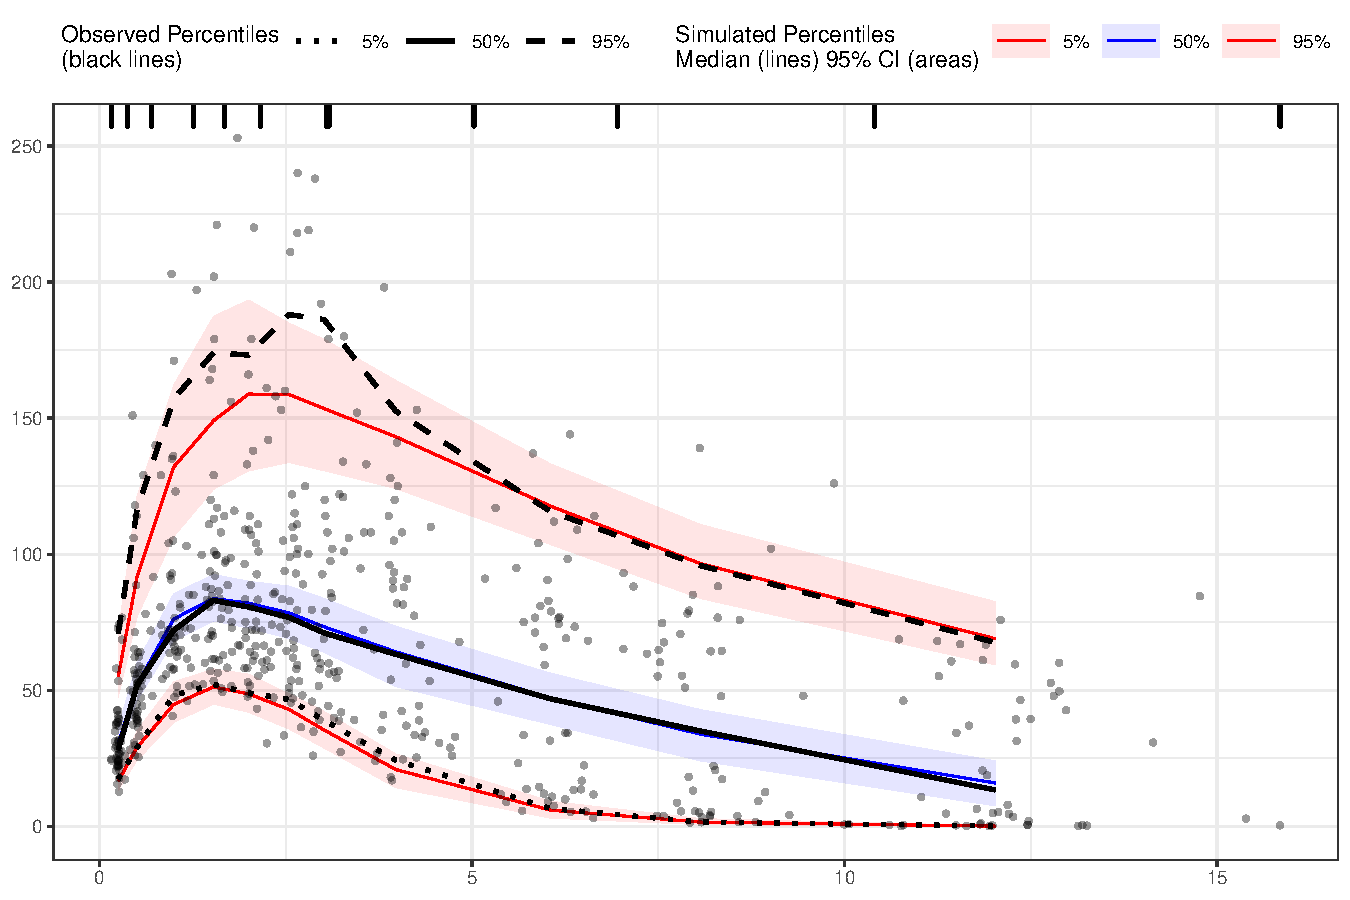
\includegraphics[width=640px]{tidyvpc_bookdown_files/figure-latex/unnamed-chunk-14-1}

\hypertarget{stratify}{%
\section{\texorpdfstring{\texttt{stratify()}}{stratify()}}\label{stratify}}

To stratify VPC include the \texttt{stratify()} function before using the \texttt{binning()} or \texttt{binless()} function and use the unquoted stratification variable(s) name as a formula. Let's stratify on \texttt{GENDER} in the data, which contains 2 levels (GENDER = ``M'', GENDER = ``F''). Include as many stratification variables as your model calls for.

\begin{Shaded}
\begin{Highlighting}[]
\NormalTok{vpc <-}\StringTok{ }\KeywordTok{observed}\NormalTok{(obs_data, }\DataTypeTok{x=}\NormalTok{TIME, }\DataTypeTok{y=}\NormalTok{DV) }\OperatorTok
\StringTok{    }\KeywordTok{simulated}\NormalTok{(sim_data, }\DataTypeTok{y=}\NormalTok{DV) }\OperatorTok
\StringTok{    }\KeywordTok{stratify}\NormalTok{(}\OperatorTok{~}\StringTok{ }\NormalTok{GENDER) }\OperatorTok
\StringTok{    }\KeywordTok{binning}\NormalTok{(}\DataTypeTok{bin =} \StringTok{"pam"}\NormalTok{, }\DataTypeTok{nbins =} \DecValTok{7}\NormalTok{) }\OperatorTok
\StringTok{    }\KeywordTok{vpcstats}\NormalTok{()}

\KeywordTok{plot}\NormalTok{(vpc)}
\end{Highlighting}
\end{Shaded}

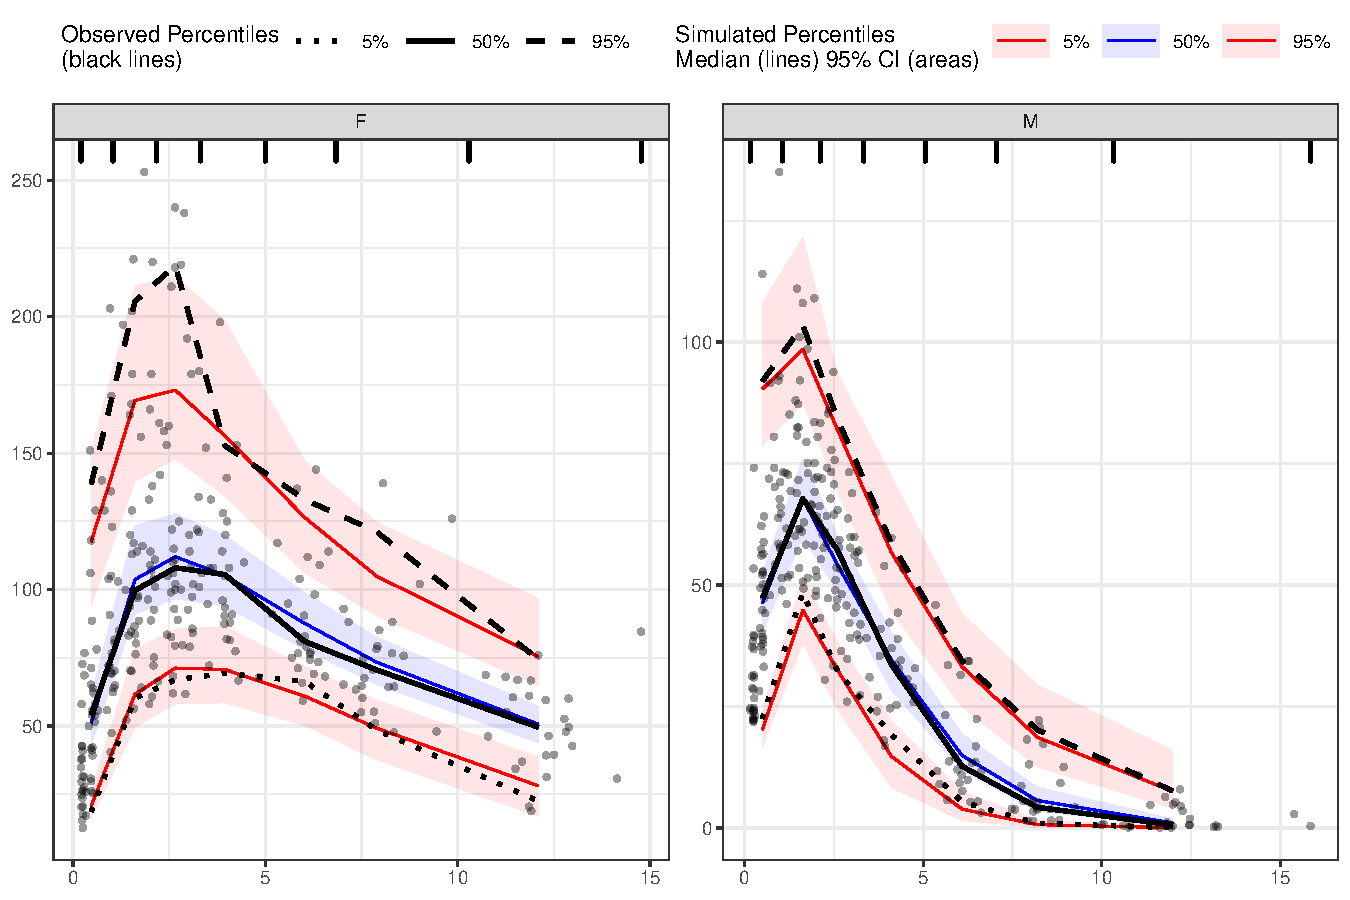
\includegraphics[width=640px]{tidyvpc_bookdown_files/figure-latex/unnamed-chunk-15-1}

Using multiple stratification variables \texttt{GENDER} and \texttt{STUDY}.

\begin{Shaded}
\begin{Highlighting}[]
\NormalTok{vpc <-}\StringTok{ }\KeywordTok{observed}\NormalTok{(obs_data, }\DataTypeTok{x=}\NormalTok{TIME, }\DataTypeTok{y=}\NormalTok{DV) }\OperatorTok
\StringTok{    }\KeywordTok{simulated}\NormalTok{(sim_data, }\DataTypeTok{y=}\NormalTok{DV) }\OperatorTok
\StringTok{    }\KeywordTok{stratify}\NormalTok{(}\OperatorTok{~}\StringTok{ }\NormalTok{GENDER }\OperatorTok{+}\StringTok{ }\NormalTok{STUDY) }\OperatorTok
\StringTok{    }\KeywordTok{binless}\NormalTok{() }\OperatorTok
\StringTok{    }\KeywordTok{vpcstats}\NormalTok{()}

\KeywordTok{plot}\NormalTok{(vpc)}
\end{Highlighting}
\end{Shaded}

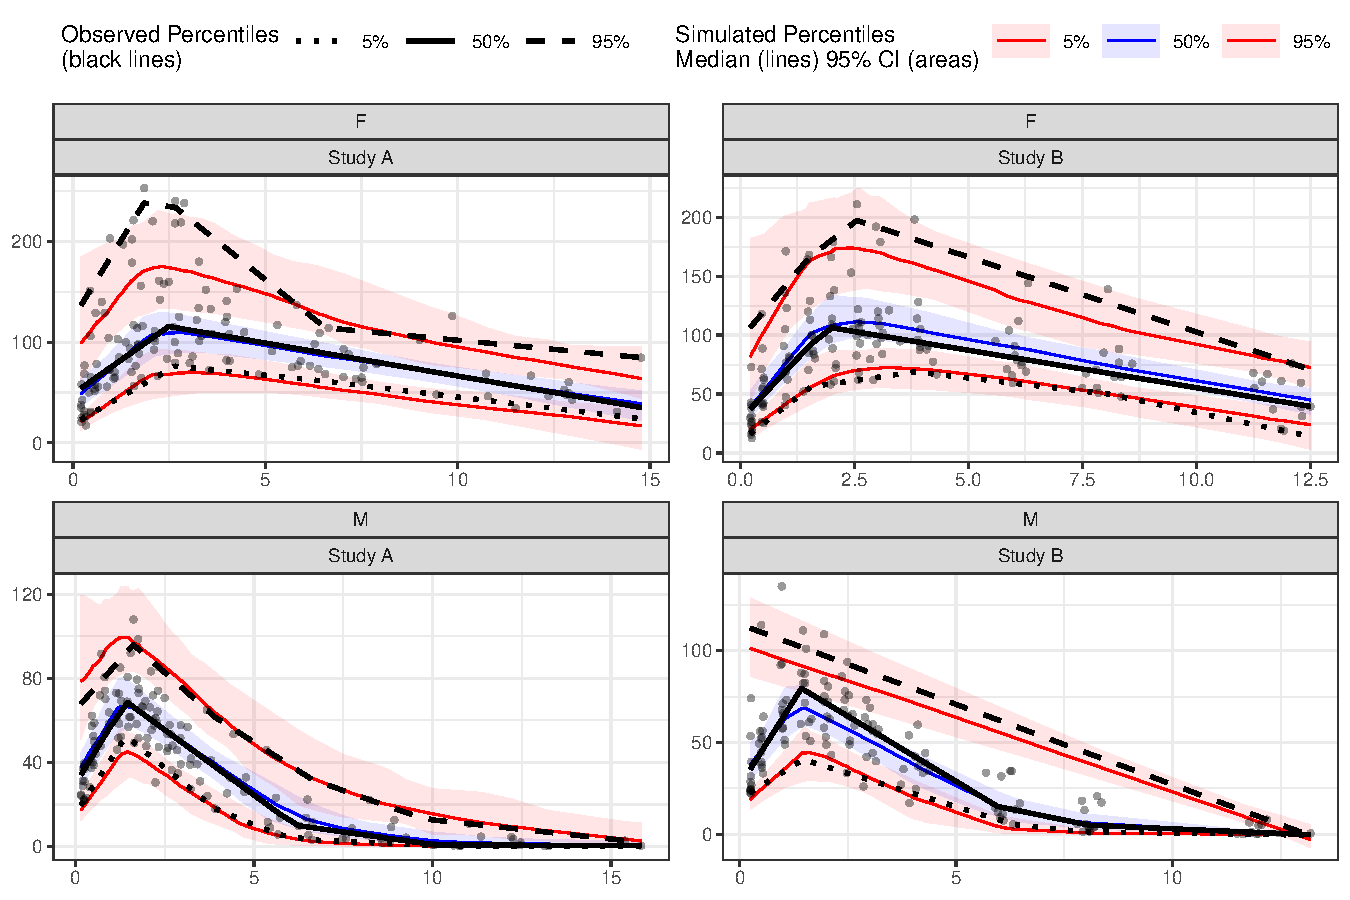
\includegraphics[width=640px]{tidyvpc_bookdown_files/figure-latex/unnamed-chunk-16-1}

\hypertarget{censoring}{%
\section{\texorpdfstring{\texttt{censoring()}}{censoring()}}\label{censoring}}

To censor observed data below lower limit of quantification (LLOQ), include the \texttt{censoring()} function after \texttt{simulated()} and use the \texttt{lloq} argument to specify either a variable in the data or specific value for censoring. The \texttt{blq} argument creates a logical TRUE/FALSE in the data that indicates whether the value is below the limit of quantification and is typically defined as rows with DV \textless{} LLOQ in the data. Using the \texttt{censoring()} function will censor only observed data below lower limit of quantification when plotting, simulated data will still be plotted.

Censoring using numeric value.

\begin{Shaded}
\begin{Highlighting}[]
\NormalTok{vpc <-}\StringTok{ }\KeywordTok{observed}\NormalTok{(obs_data, }\DataTypeTok{x=}\NormalTok{TIME, }\DataTypeTok{y=}\NormalTok{DV) }\OperatorTok
\StringTok{    }\KeywordTok{simulated}\NormalTok{(sim_data, }\DataTypeTok{y=}\NormalTok{DV) }\OperatorTok
\StringTok{    }\KeywordTok{censoring}\NormalTok{(}\DataTypeTok{blq=}\NormalTok{(DV }\OperatorTok{<}\StringTok{ }\DecValTok{25}\NormalTok{), }\DataTypeTok{lloq=}\DecValTok{25}\NormalTok{) }\OperatorTok
\StringTok{    }\KeywordTok{binning}\NormalTok{(}\DataTypeTok{bin =} \StringTok{"jenks"}\NormalTok{, }\DataTypeTok{nbins =} \DecValTok{5}\NormalTok{) }\OperatorTok
\StringTok{    }\KeywordTok{vpcstats}\NormalTok{()}

\KeywordTok{plot}\NormalTok{(vpc)}
\end{Highlighting}
\end{Shaded}

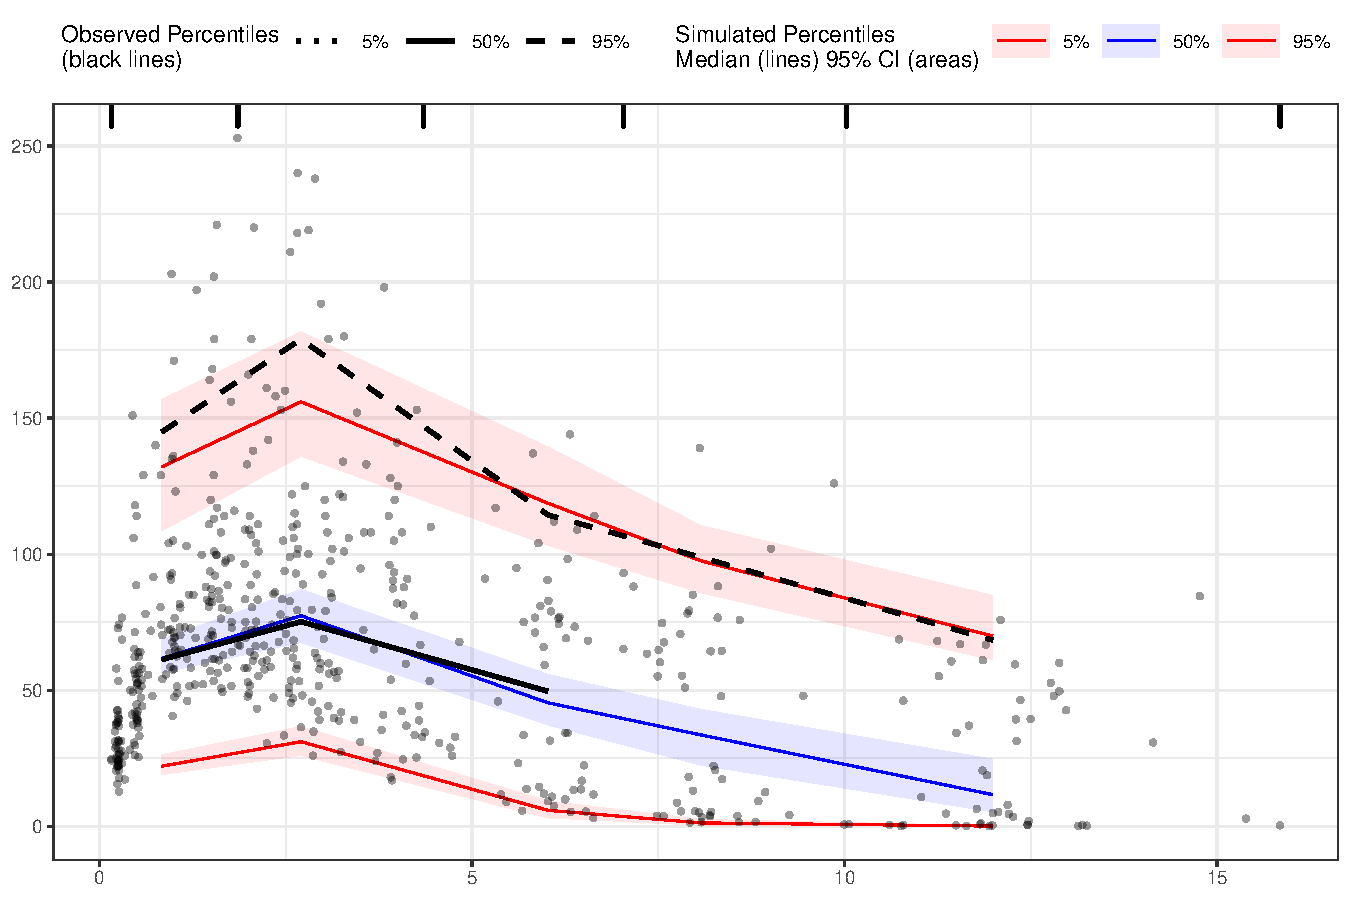
\includegraphics[width=640px]{tidyvpc_bookdown_files/figure-latex/unnamed-chunk-17-1}

Censoring using \texttt{LLOQ} variable in the data.

First, let's add an LLOQ variable to the observed data.

\begin{Shaded}
\begin{Highlighting}[]
\NormalTok{obs_data}\OperatorTok{$}\NormalTok{LLOQ <-}\StringTok{ }\DecValTok{50}
\end{Highlighting}
\end{Shaded}

Then we'll specify lower limit of quantification as the unquoted variable name in our data \texttt{LLOQ}. Let's also provide our own lambda values.

\begin{Shaded}
\begin{Highlighting}[]
\NormalTok{vpc <-}\StringTok{ }\KeywordTok{observed}\NormalTok{(obs_data, }\DataTypeTok{x=}\NormalTok{TIME, }\DataTypeTok{y=}\NormalTok{DV) }\OperatorTok
\StringTok{    }\KeywordTok{simulated}\NormalTok{(sim_data, }\DataTypeTok{y=}\NormalTok{DV) }\OperatorTok
\StringTok{    }\KeywordTok{censoring}\NormalTok{(}\DataTypeTok{blq=}\NormalTok{(DV }\OperatorTok{<}\StringTok{ }\NormalTok{LLOQ), }\DataTypeTok{lloq=}\NormalTok{LLOQ) }\OperatorTok
\StringTok{    }\KeywordTok{binless}\NormalTok{(}\DataTypeTok{optimize =} \OtherTok{FALSE}\NormalTok{, }\DataTypeTok{lambda =} \KeywordTok{c}\NormalTok{(}\FloatTok{1.5}\NormalTok{, }\FloatTok{2.5}\NormalTok{, }\FloatTok{1.7}\NormalTok{)) }\OperatorTok
\StringTok{    }\KeywordTok{vpcstats}\NormalTok{()}

\KeywordTok{plot}\NormalTok{(vpc)}
\end{Highlighting}
\end{Shaded}

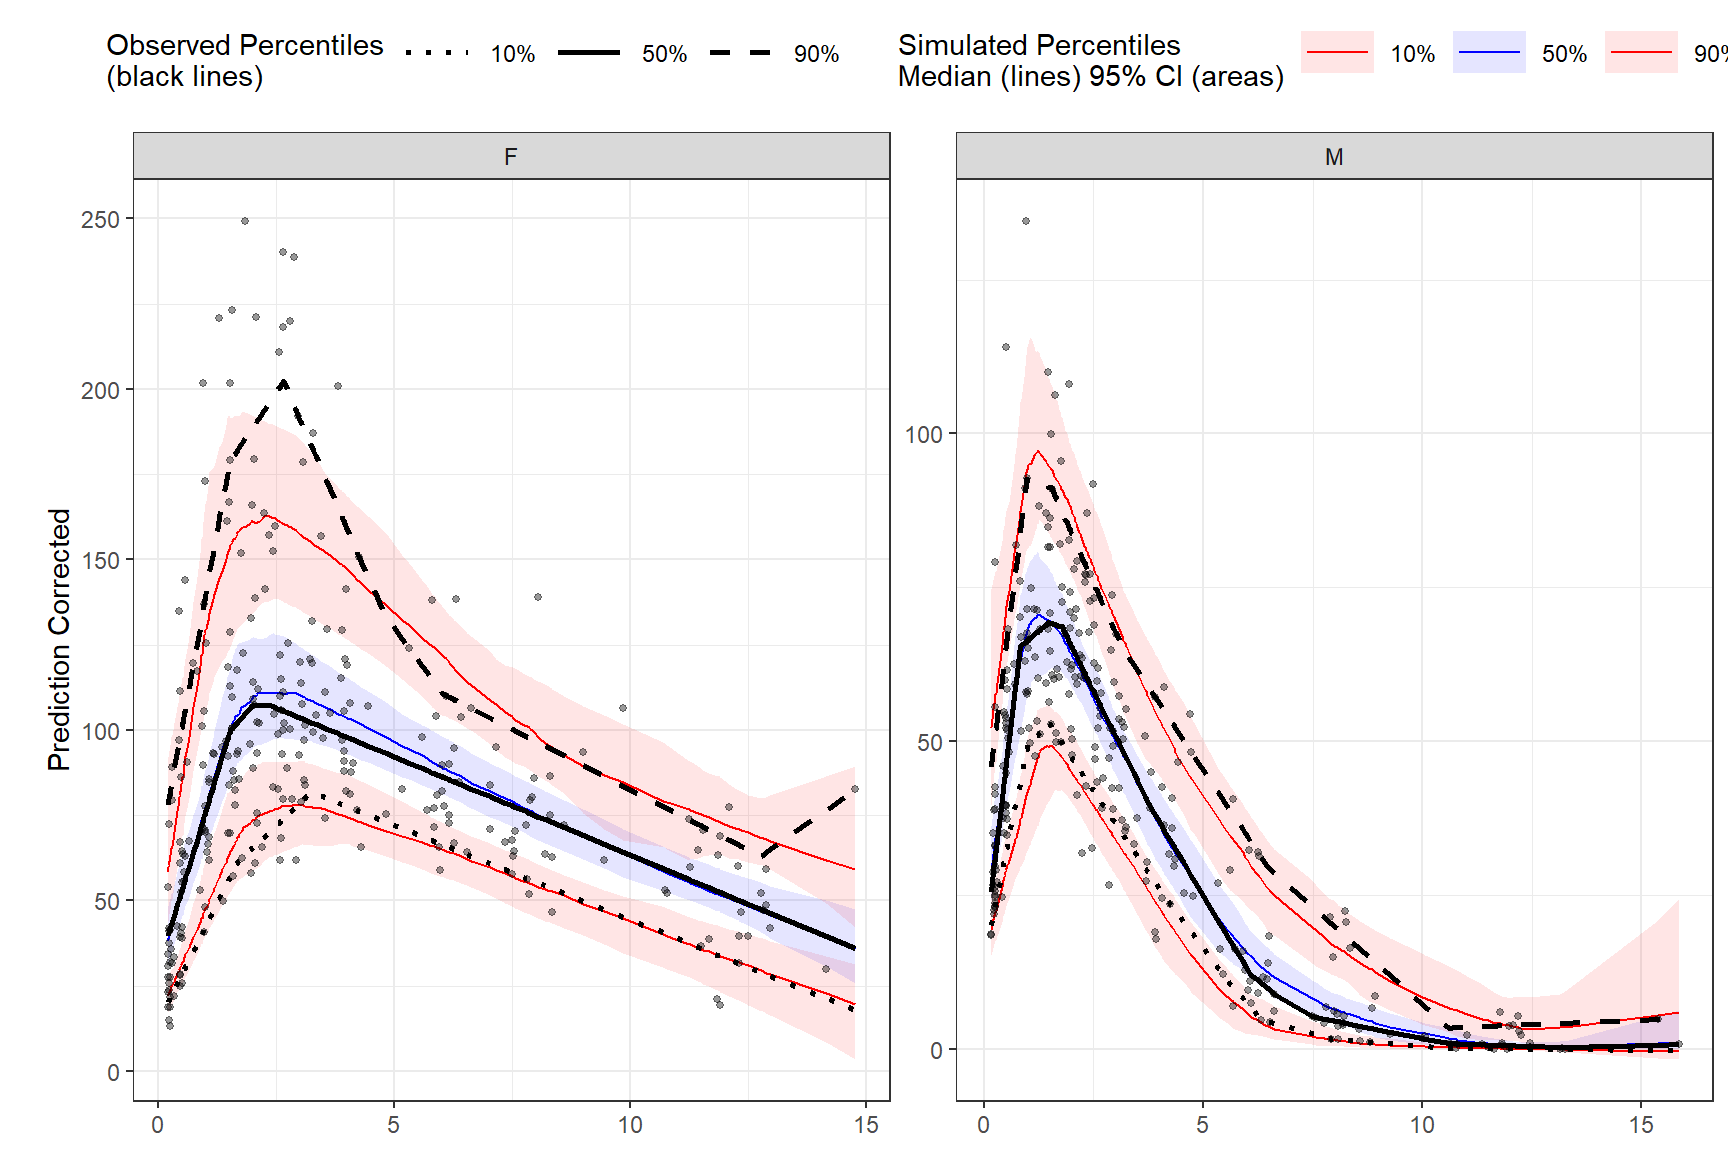
\includegraphics[width=640px]{tidyvpc_bookdown_files/figure-latex/unnamed-chunk-19-1}

The \texttt{tidyvpc} package also allows you to use different LLOQ for each level of stratification variable. We'll set an \texttt{LLOQ} value of \texttt{50} for \texttt{Study\ A} and \texttt{25} for \texttt{Study\ B} and calculate statistics at 5\%, 50\%, 90\% quantiles.

\begin{Shaded}
\begin{Highlighting}[]
\NormalTok{obs_data}\OperatorTok{$}\NormalTok{LLOQ <-}\StringTok{ }\KeywordTok{ifelse}\NormalTok{(obs_data}\OperatorTok{$}\NormalTok{STUDY }\OperatorTok{==}\StringTok{ "Study A"}\NormalTok{, }\DecValTok{50}\NormalTok{, }\DecValTok{25}\NormalTok{)}

\NormalTok{vpc <-}\StringTok{ }\KeywordTok{observed}\NormalTok{(obs_data, }\DataTypeTok{x=}\NormalTok{TIME, }\DataTypeTok{y=}\NormalTok{DV) }\OperatorTok
\StringTok{    }\KeywordTok{simulated}\NormalTok{(sim_data, }\DataTypeTok{y=}\NormalTok{DV) }\OperatorTok
\StringTok{    }\KeywordTok{censoring}\NormalTok{(}\DataTypeTok{blq=}\NormalTok{(DV }\OperatorTok{<}\StringTok{ }\NormalTok{LLOQ), }\DataTypeTok{lloq=}\NormalTok{LLOQ) }\OperatorTok
\StringTok{    }\KeywordTok{stratify}\NormalTok{(}\OperatorTok{~}\StringTok{ }\NormalTok{STUDY) }\OperatorTok
\StringTok{    }\KeywordTok{binning}\NormalTok{(}\DataTypeTok{bin =} \StringTok{"pam"}\NormalTok{, }\DataTypeTok{nbins =} \DecValTok{4}\NormalTok{) }\OperatorTok
\StringTok{    }\KeywordTok{vpcstats}\NormalTok{(}\DataTypeTok{qpred =} \KeywordTok{c}\NormalTok{(}\FloatTok{0.1}\NormalTok{, }\FloatTok{0.5}\NormalTok{, }\FloatTok{0.9}\NormalTok{))}

\KeywordTok{plot}\NormalTok{(vpc)}
\end{Highlighting}
\end{Shaded}

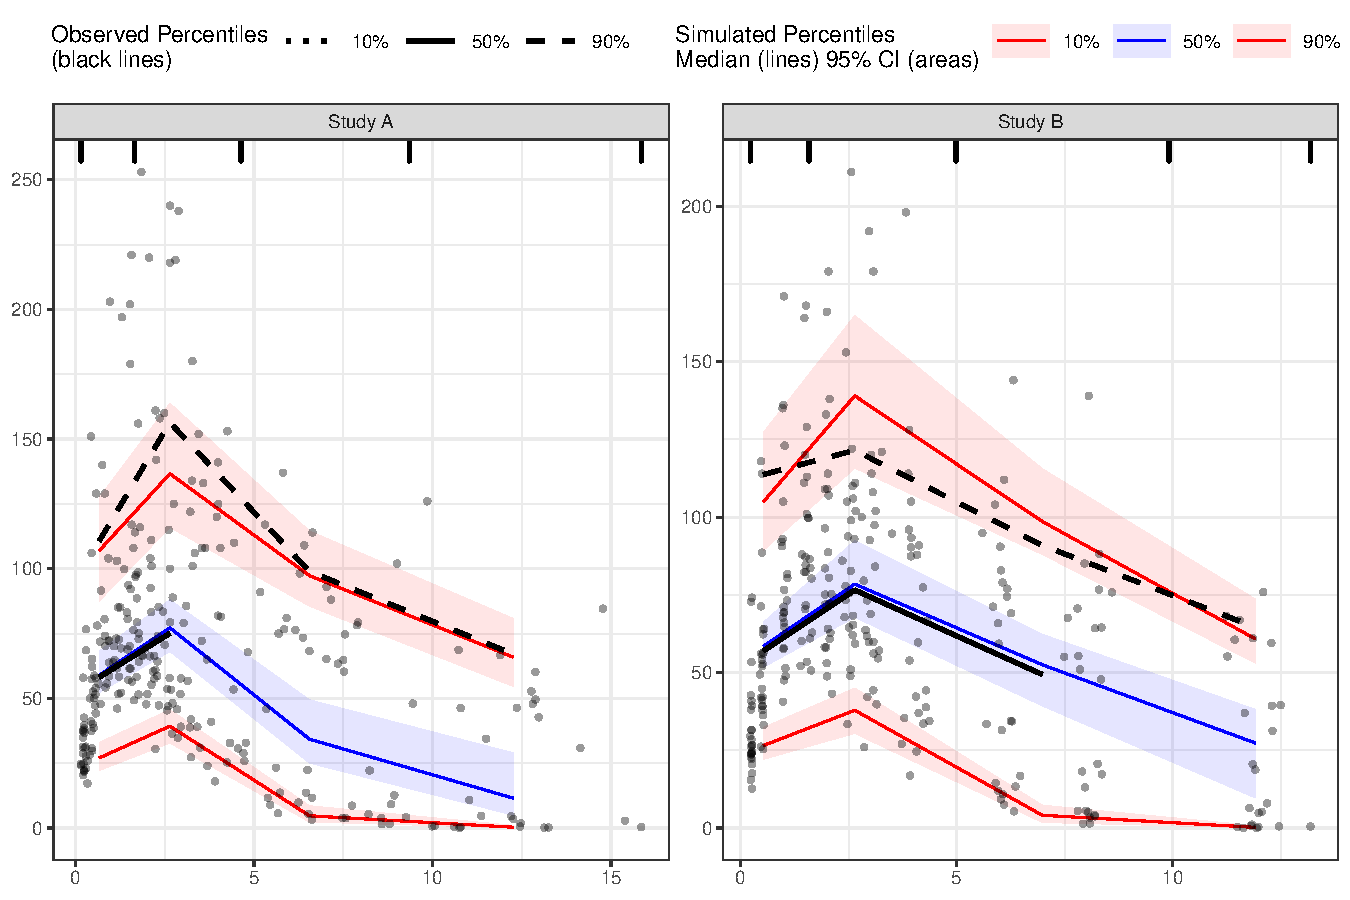
\includegraphics[width=640px]{tidyvpc_bookdown_files/figure-latex/unnamed-chunk-20-1}

\hypertarget{predcorrect}{%
\section{\texorpdfstring{\texttt{predcorrect()}}{predcorrect()}}\label{predcorrect}}

To derive a prediction corrected VPC (pcVPC) use the \texttt{predcorrect()} function. The \texttt{predcorrect()} function takes one required argument \texttt{pred} which should be the unquoted variable name of the population prediction variable in the data. If using binning methods, the \texttt{predcorrect()} function should be called \emph{after} \texttt{binning()}, however, if performing LOESS pcVPC for \texttt{binless()} methods, use \texttt{predcorrect()} \emph{before} calling \texttt{binless()} and set \texttt{binless(loess.ypc\ =\ TRUE)}. Note: if model was fit using log scale of DV make sure to include the argument \texttt{log\ =\ TRUE} in \texttt{predcorrect()} to perform the appropriate prediction correction calculation.

Prediction corrected using binning methods.

\begin{Shaded}
\begin{Highlighting}[]
\NormalTok{vpc <-}\StringTok{ }\KeywordTok{observed}\NormalTok{(obs_data, }\DataTypeTok{x=}\NormalTok{TIME, }\DataTypeTok{y=}\NormalTok{DV) }\OperatorTok
\StringTok{    }\KeywordTok{simulated}\NormalTok{(sim_data, }\DataTypeTok{y=}\NormalTok{DV) }\OperatorTok
\StringTok{    }\KeywordTok{stratify}\NormalTok{(}\OperatorTok{~}\NormalTok{GENDER) }\OperatorTok
\StringTok{    }\KeywordTok{binning}\NormalTok{(}\DataTypeTok{bin =}\NormalTok{ NTIME) }\OperatorTok
\StringTok{    }\KeywordTok{predcorrect}\NormalTok{(}\DataTypeTok{pred=}\NormalTok{PRED) }\OperatorTok
\StringTok{    }\KeywordTok{vpcstats}\NormalTok{()}

\KeywordTok{plot}\NormalTok{(vpc)}
\end{Highlighting}
\end{Shaded}

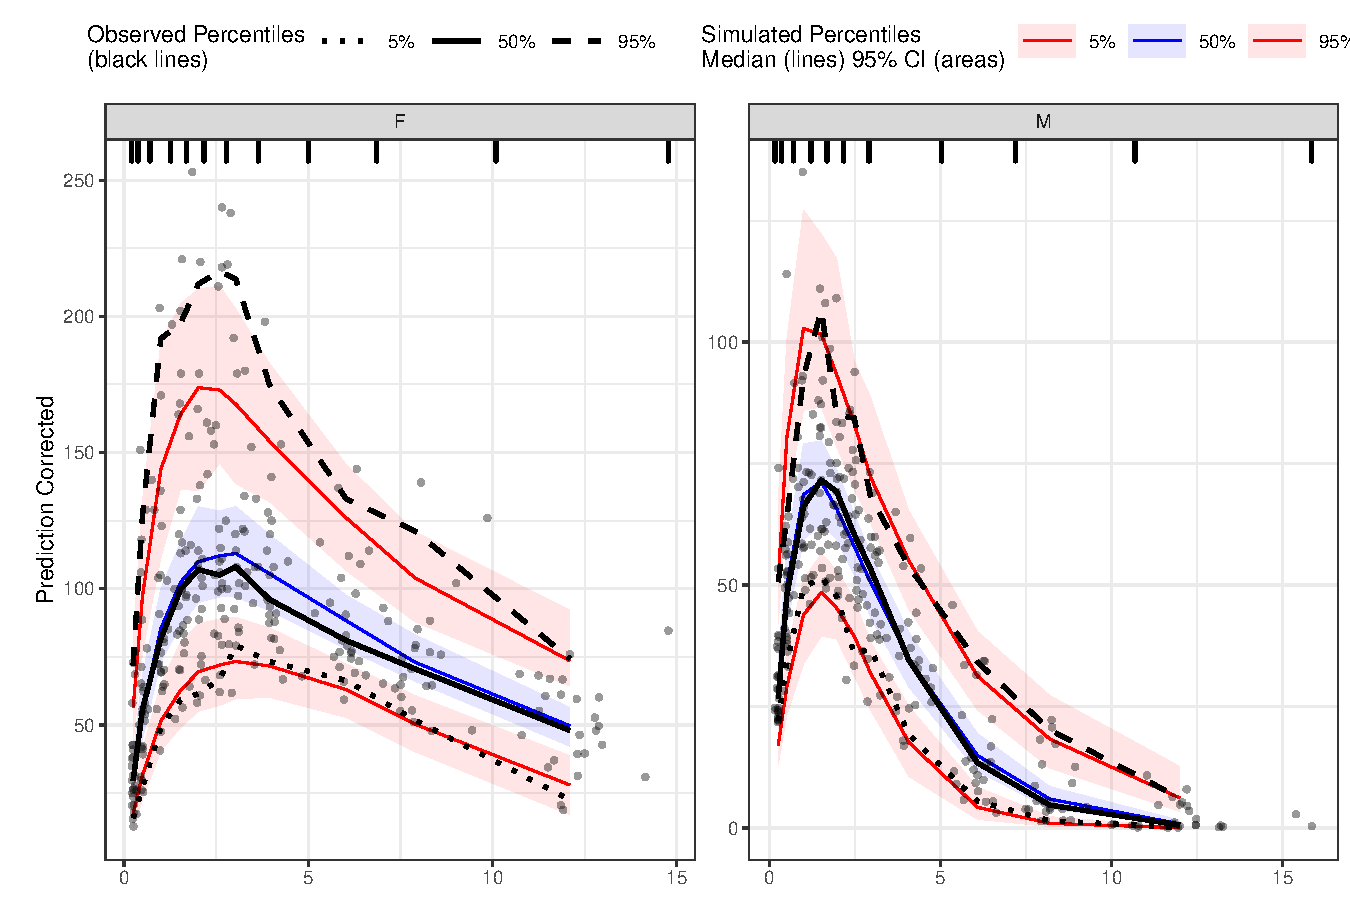
\includegraphics[width=640px]{tidyvpc_bookdown_files/figure-latex/unnamed-chunk-21-1}

LOESS prediction corrected using binless method for 10\%, 50\%, 90\% quantiles. If \texttt{optimize\ =\ TRUE}, the LOESS smoothing parameter, span, will be automatically optimize using AIC. Note: \texttt{predcorrect()} must be called before \texttt{binless()} if setting \texttt{loess.ypc\ =\ TRUE}.

\begin{Shaded}
\begin{Highlighting}[]
\NormalTok{vpc <-}\StringTok{ }\KeywordTok{observed}\NormalTok{(obs_data, }\DataTypeTok{x=}\NormalTok{TIME, }\DataTypeTok{y=}\NormalTok{DV) }\OperatorTok
\StringTok{    }\KeywordTok{simulated}\NormalTok{(sim_data, }\DataTypeTok{y=}\NormalTok{DV) }\OperatorTok
\StringTok{    }\KeywordTok{stratify}\NormalTok{(}\OperatorTok{~}\NormalTok{GENDER) }\OperatorTok
\StringTok{    }\KeywordTok{predcorrect}\NormalTok{(}\DataTypeTok{pred=}\NormalTok{PRED) }\OperatorTok
\StringTok{    }\KeywordTok{binless}\NormalTok{(}\DataTypeTok{qpred =} \KeywordTok{c}\NormalTok{(}\FloatTok{0.1}\NormalTok{, }\FloatTok{0.5}\NormalTok{, }\FloatTok{0.9}\NormalTok{), }\DataTypeTok{optimize =} \OtherTok{TRUE}\NormalTok{, }\DataTypeTok{loess.ypc =} \OtherTok{TRUE}\NormalTok{) }\OperatorTok
\StringTok{    }\KeywordTok{vpcstats}\NormalTok{()}

\KeywordTok{plot}\NormalTok{(vpc)}
\end{Highlighting}
\end{Shaded}

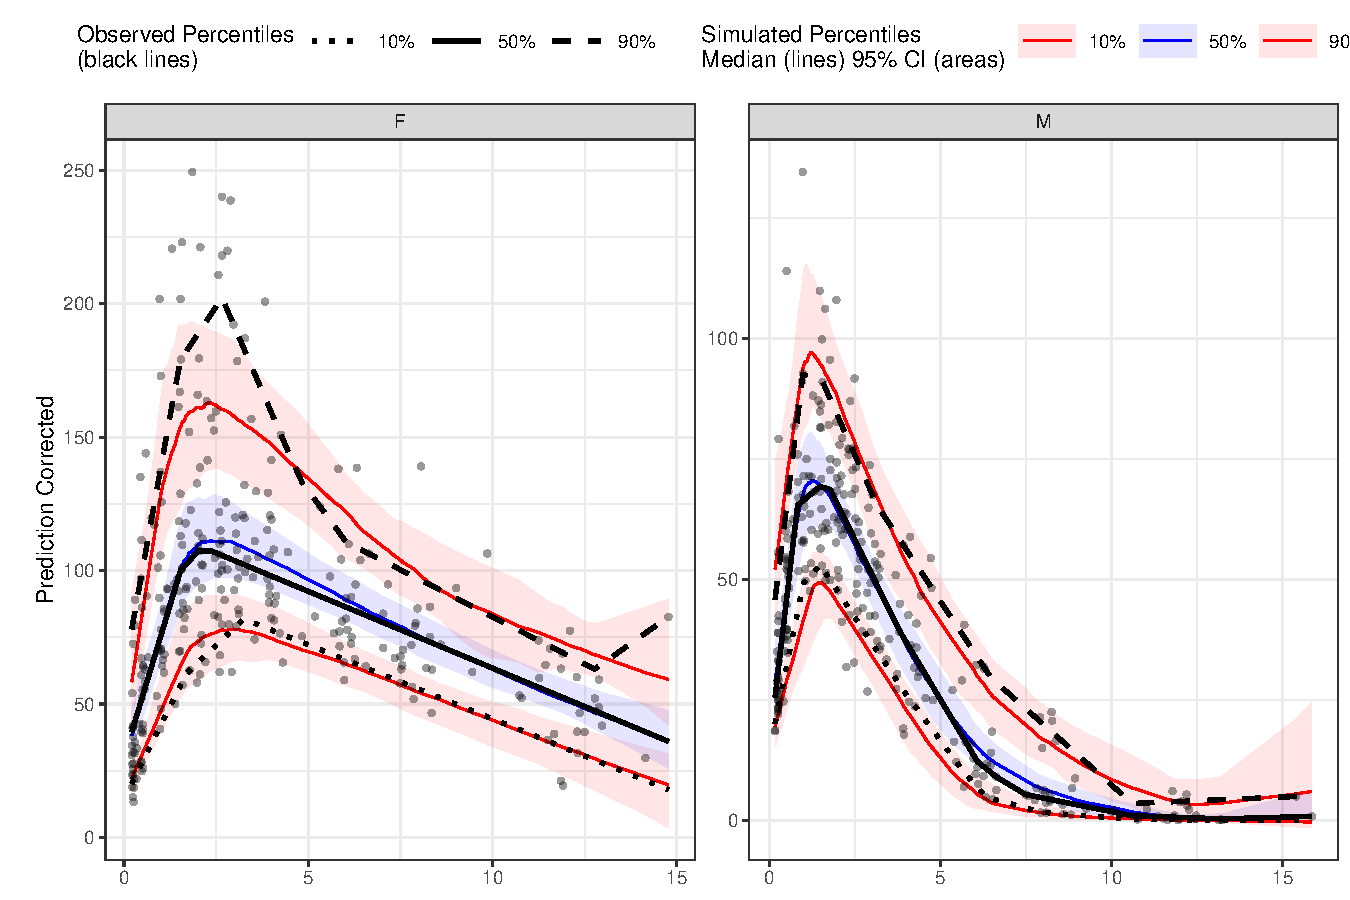
\includegraphics[width=640px]{tidyvpc_bookdown_files/figure-latex/unnamed-chunk-22-1}

To specify your own span value LOESS pcVPC instead of optimizing with AIC, use the \texttt{span} argument in the \texttt{binless} function. Span should be a numeric between {[}0,1{]}, with higher values providing a smoother fit. Remember, to also include the smoothing parameters for AQR by using the \texttt{lambda} argument and set \texttt{optimize\ =\ FALSE}.

\begin{Shaded}
\begin{Highlighting}[]
\NormalTok{vpc <-}\StringTok{ }\KeywordTok{observed}\NormalTok{(obs_data, }\DataTypeTok{x=}\NormalTok{TIME, }\DataTypeTok{y=}\NormalTok{DV) }\OperatorTok
\StringTok{    }\KeywordTok{simulated}\NormalTok{(sim_data, }\DataTypeTok{y=}\NormalTok{DV) }\OperatorTok
\StringTok{    }\KeywordTok{predcorrect}\NormalTok{(}\DataTypeTok{pred=}\NormalTok{PRED) }\OperatorTok
\StringTok{    }\KeywordTok{binless}\NormalTok{(}\DataTypeTok{optimize =} \OtherTok{FALSE}\NormalTok{, }\DataTypeTok{lambda =} \KeywordTok{c}\NormalTok{(.}\DecValTok{95}\NormalTok{,}\DecValTok{3}\NormalTok{,}\FloatTok{1.2}\NormalTok{), }\DataTypeTok{loess.ypc =} \OtherTok{TRUE}\NormalTok{, }\DataTypeTok{span =} \FloatTok{.6}\NormalTok{) }\OperatorTok
\StringTok{    }\KeywordTok{vpcstats}\NormalTok{()}

\KeywordTok{plot}\NormalTok{(vpc)}
\end{Highlighting}
\end{Shaded}

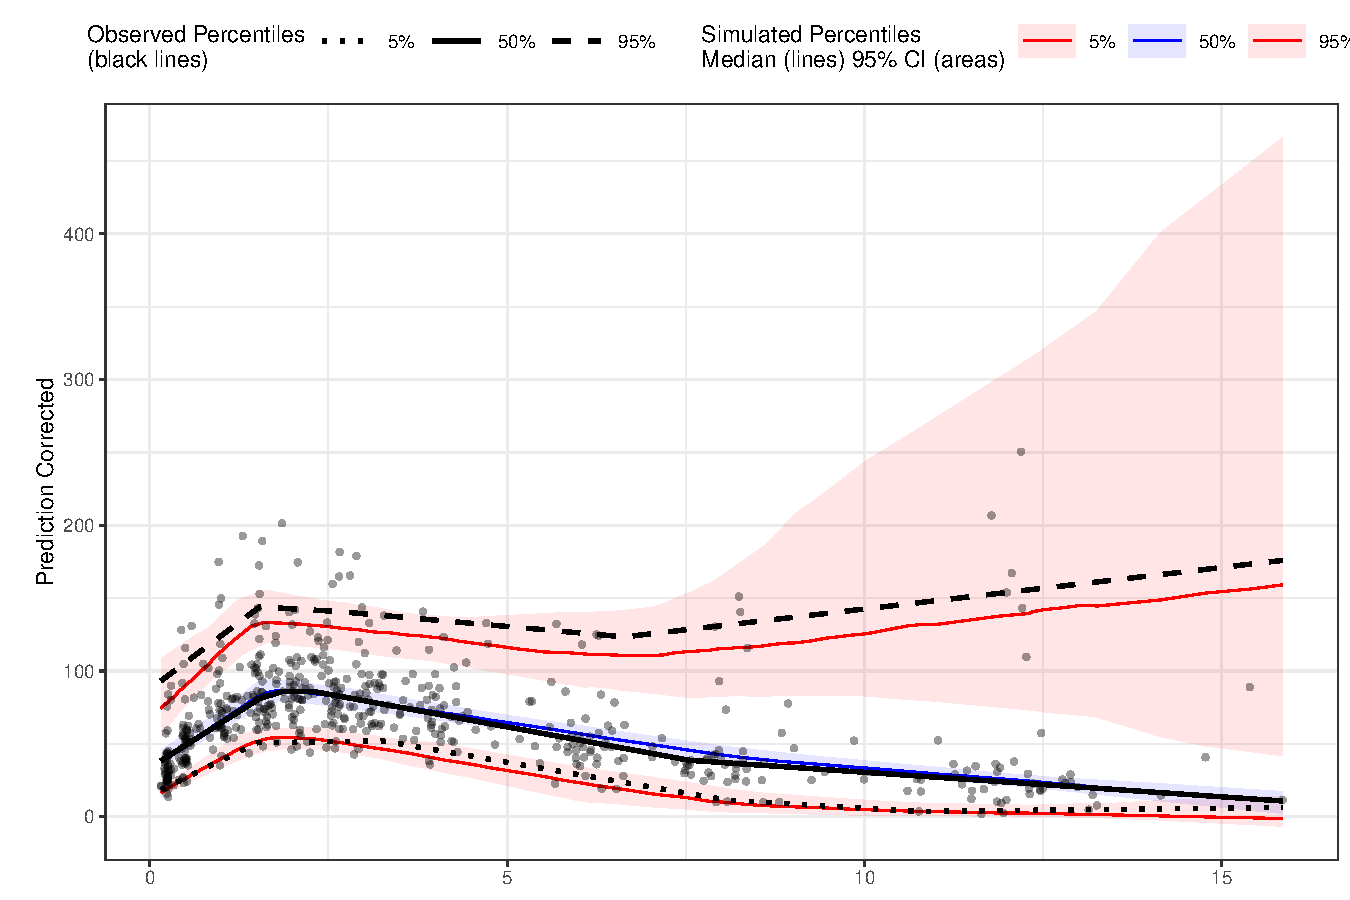
\includegraphics[width=640px]{tidyvpc_bookdown_files/figure-latex/unnamed-chunk-23-1}

\hypertarget{advanced}{%
\chapter{Advanced}\label{advanced}}

The following chapter provides advanced use cases of the \texttt{tidyvpc} package.

\hypertarget{binning-by-strata}{%
\section{Binning by Strata}\label{binning-by-strata}}

To use different binning methods for different stratification variables, and/or for each level of stratification variable, use multiple calls to the \texttt{binning()} function in combination with the \texttt{stratum} argument. Make sure to set \texttt{by.strata\ =\ T}

\begin{Shaded}
\begin{Highlighting}[]
\NormalTok{vpc <-}\StringTok{ }\KeywordTok{observed}\NormalTok{(obs_data, }\DataTypeTok{x=}\NormalTok{TIME, }\DataTypeTok{y=}\NormalTok{DV) }\OperatorTok
\StringTok{    }\KeywordTok{simulated}\NormalTok{(sim_data, }\DataTypeTok{y=}\NormalTok{DV) }\OperatorTok
\StringTok{    }\KeywordTok{stratify}\NormalTok{(}\OperatorTok{~}\StringTok{ }\NormalTok{GENDER }\OperatorTok{+}\StringTok{ }\NormalTok{STUDY) }\OperatorTok
\StringTok{    }\KeywordTok{binning}\NormalTok{(}\DataTypeTok{stratum =} \KeywordTok{list}\NormalTok{(}\DataTypeTok{GENDER =} \StringTok{"M"}\NormalTok{, }\DataTypeTok{STUDY =} \StringTok{"Study A"}\NormalTok{), }\DataTypeTok{bin =} \StringTok{"jenks"}\NormalTok{, }\DataTypeTok{nbins =} \DecValTok{5}\NormalTok{, }\DataTypeTok{by.strata =}\NormalTok{ T) }\OperatorTok
\StringTok{    }\KeywordTok{binning}\NormalTok{(}\DataTypeTok{stratum =} \KeywordTok{list}\NormalTok{(}\DataTypeTok{GENDER =} \StringTok{"F"}\NormalTok{, }\DataTypeTok{STUDY =} \StringTok{"Study A"}\NormalTok{), }\DataTypeTok{bin =} \StringTok{"centers"}\NormalTok{, }\DataTypeTok{centers =} \KeywordTok{c}\NormalTok{(}\FloatTok{0.5}\NormalTok{,}\DecValTok{3}\NormalTok{,}\DecValTok{5}\NormalTok{,}\DecValTok{10}\NormalTok{,}\DecValTok{15}\NormalTok{), }\DataTypeTok{by.strata =}\NormalTok{ T) }\OperatorTok
\StringTok{    }\KeywordTok{binning}\NormalTok{(}\DataTypeTok{stratum =} \KeywordTok{list}\NormalTok{(}\DataTypeTok{GENDER =} \StringTok{"M"}\NormalTok{, }\DataTypeTok{STUDY =} \StringTok{"Study B"}\NormalTok{), }\DataTypeTok{bin =} \StringTok{"kmeans"}\NormalTok{, }\DataTypeTok{by.strata =}\NormalTok{ T) }\OperatorTok
\StringTok{    }\KeywordTok{binning}\NormalTok{(}\DataTypeTok{stratum =} \KeywordTok{list}\NormalTok{(}\DataTypeTok{GENDER =} \StringTok{"F"}\NormalTok{, }\DataTypeTok{STUDY =} \StringTok{"Study B"}\NormalTok{), }\DataTypeTok{bin =} \StringTok{"pam"}\NormalTok{, }\DataTypeTok{nbins =} \DecValTok{5}\NormalTok{, }\DataTypeTok{by.strata =}\NormalTok{ T) }\OperatorTok
\StringTok{    }\KeywordTok{predcorrect}\NormalTok{(}\DataTypeTok{pred=}\NormalTok{PRED) }\OperatorTok
\StringTok{    }\KeywordTok{vpcstats}\NormalTok{()}

\KeywordTok{plot}\NormalTok{(vpc)}
\end{Highlighting}
\end{Shaded}

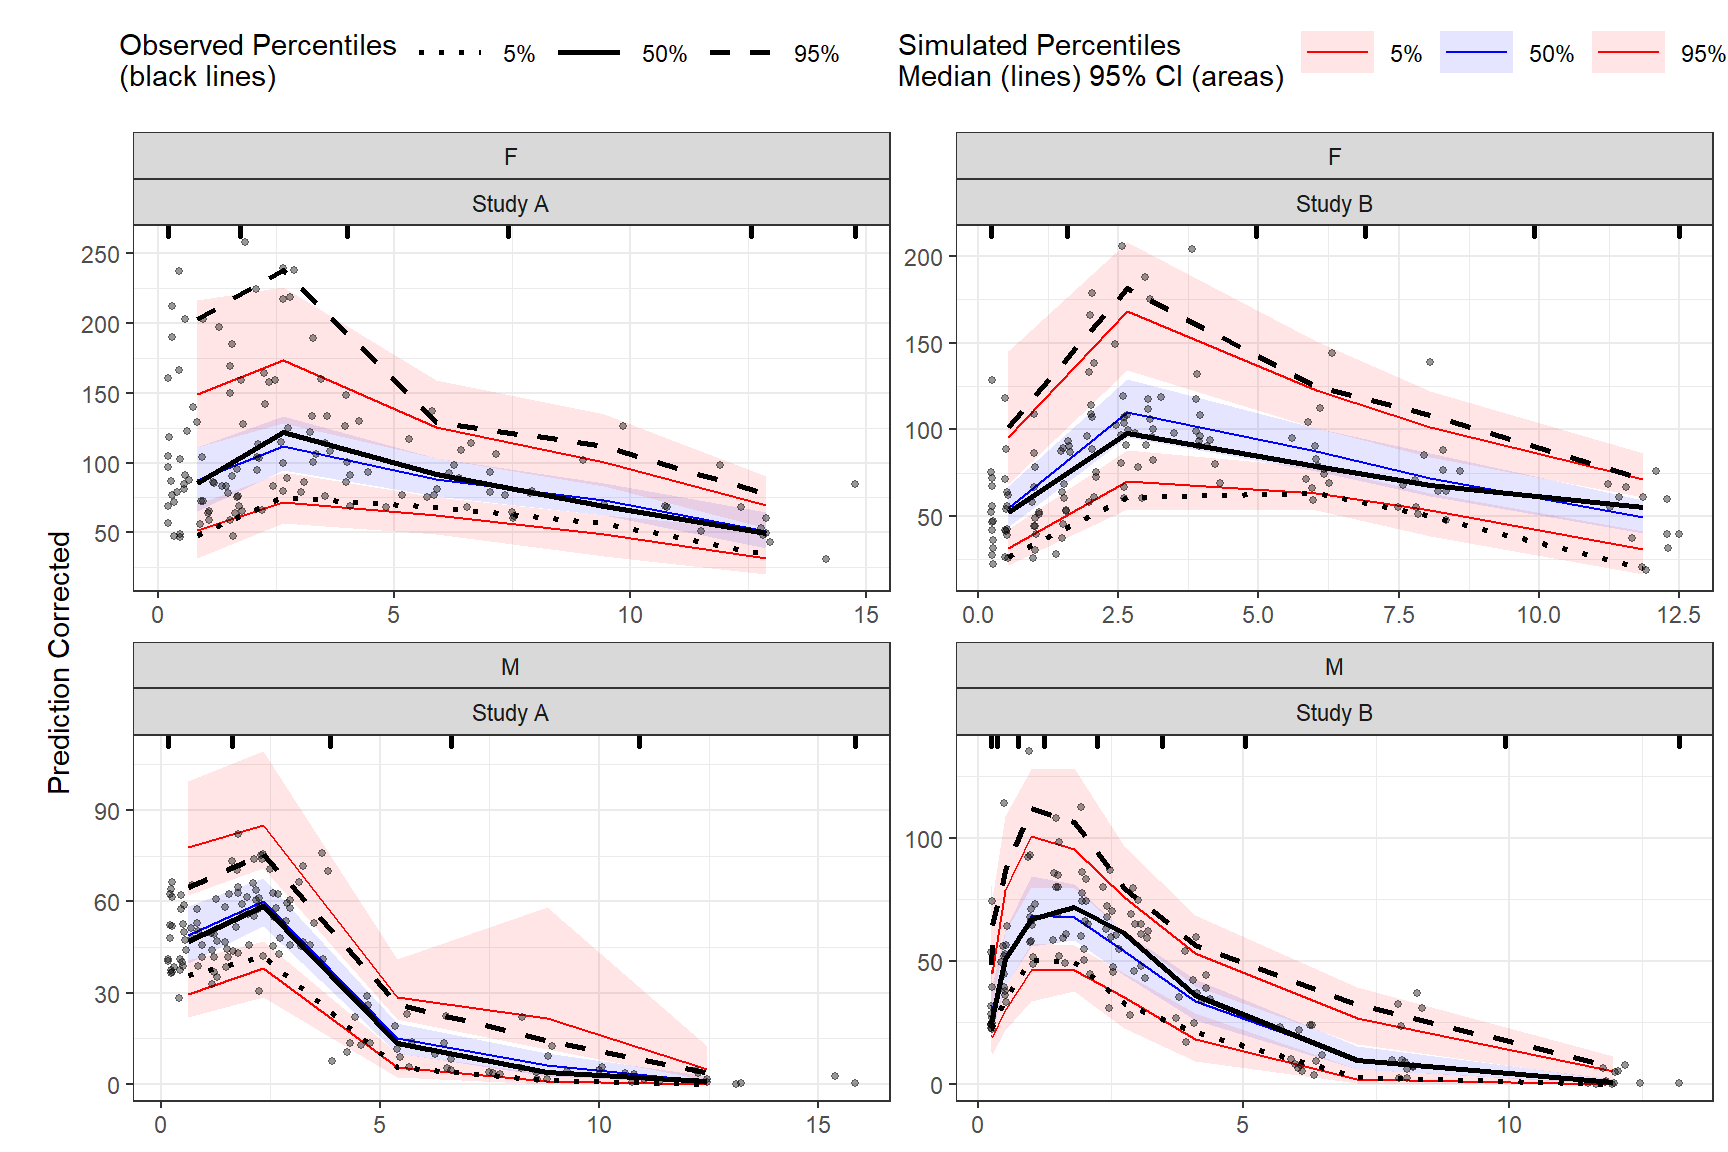
\includegraphics[width=640px]{tidyvpc_bookdown_files/figure-latex/bin-strata-1}

\hypertarget{binless-by-strata}{%
\section{Binless by Strata}\label{binless-by-strata}}

To use different smoothing parameters for each level of stratification variable if using the \texttt{binless()} function use a single call of the \texttt{binless()} function and include a \texttt{data.frame} with the column names of stratification variable and corresponding level. To use different \texttt{span} values for each level of stratification variable use a vector the length of n levels of strata. Note: If using more than one stratification variable with the \texttt{binless()} function you must set \texttt{optimize\ =\ TRUE} and optimize lambda and span using AIC.

\begin{Shaded}
\begin{Highlighting}[]
\NormalTok{new_lambda =}\StringTok{ }\KeywordTok{data.frame}\NormalTok{(}\DataTypeTok{GENDER_F =} \KeywordTok{c}\NormalTok{(}\DecValTok{2}\NormalTok{,}\DecValTok{4}\NormalTok{,}\DecValTok{2}\NormalTok{), }\DataTypeTok{GENDER_M =} \KeywordTok{c}\NormalTok{(}\FloatTok{1.9}\NormalTok{,}\DecValTok{3}\NormalTok{,}\FloatTok{2.25}\NormalTok{) )}

\NormalTok{vpc <-}\StringTok{ }\KeywordTok{observed}\NormalTok{(obs_data, }\DataTypeTok{x=}\NormalTok{TIME, }\DataTypeTok{y=}\NormalTok{DV) }\OperatorTok
\StringTok{    }\KeywordTok{simulated}\NormalTok{(sim_data, }\DataTypeTok{y=}\NormalTok{DV) }\OperatorTok
\StringTok{    }\KeywordTok{stratify}\NormalTok{(}\OperatorTok{~}\StringTok{ }\NormalTok{GENDER) }\OperatorTok
\StringTok{    }\KeywordTok{predcorrect}\NormalTok{(}\DataTypeTok{pred=}\NormalTok{PRED) }\OperatorTok
\StringTok{    }\KeywordTok{binless}\NormalTok{(}\DataTypeTok{qpred =} \KeywordTok{c}\NormalTok{(}\FloatTok{0.1}\NormalTok{, }\FloatTok{0.5}\NormalTok{, }\FloatTok{0.9}\NormalTok{), }\DataTypeTok{optimize =} \OtherTok{FALSE}\NormalTok{, }\DataTypeTok{lambda =}\NormalTok{ new_lambda, }\DataTypeTok{loess.ypc =} \OtherTok{TRUE}\NormalTok{, }\DataTypeTok{span =} \KeywordTok{c}\NormalTok{(.}\DecValTok{6}\NormalTok{, }\FloatTok{.85}\NormalTok{)) }\OperatorTok
\StringTok{    }\KeywordTok{vpcstats}\NormalTok{()}

\KeywordTok{plot}\NormalTok{(vpc)}
\end{Highlighting}
\end{Shaded}

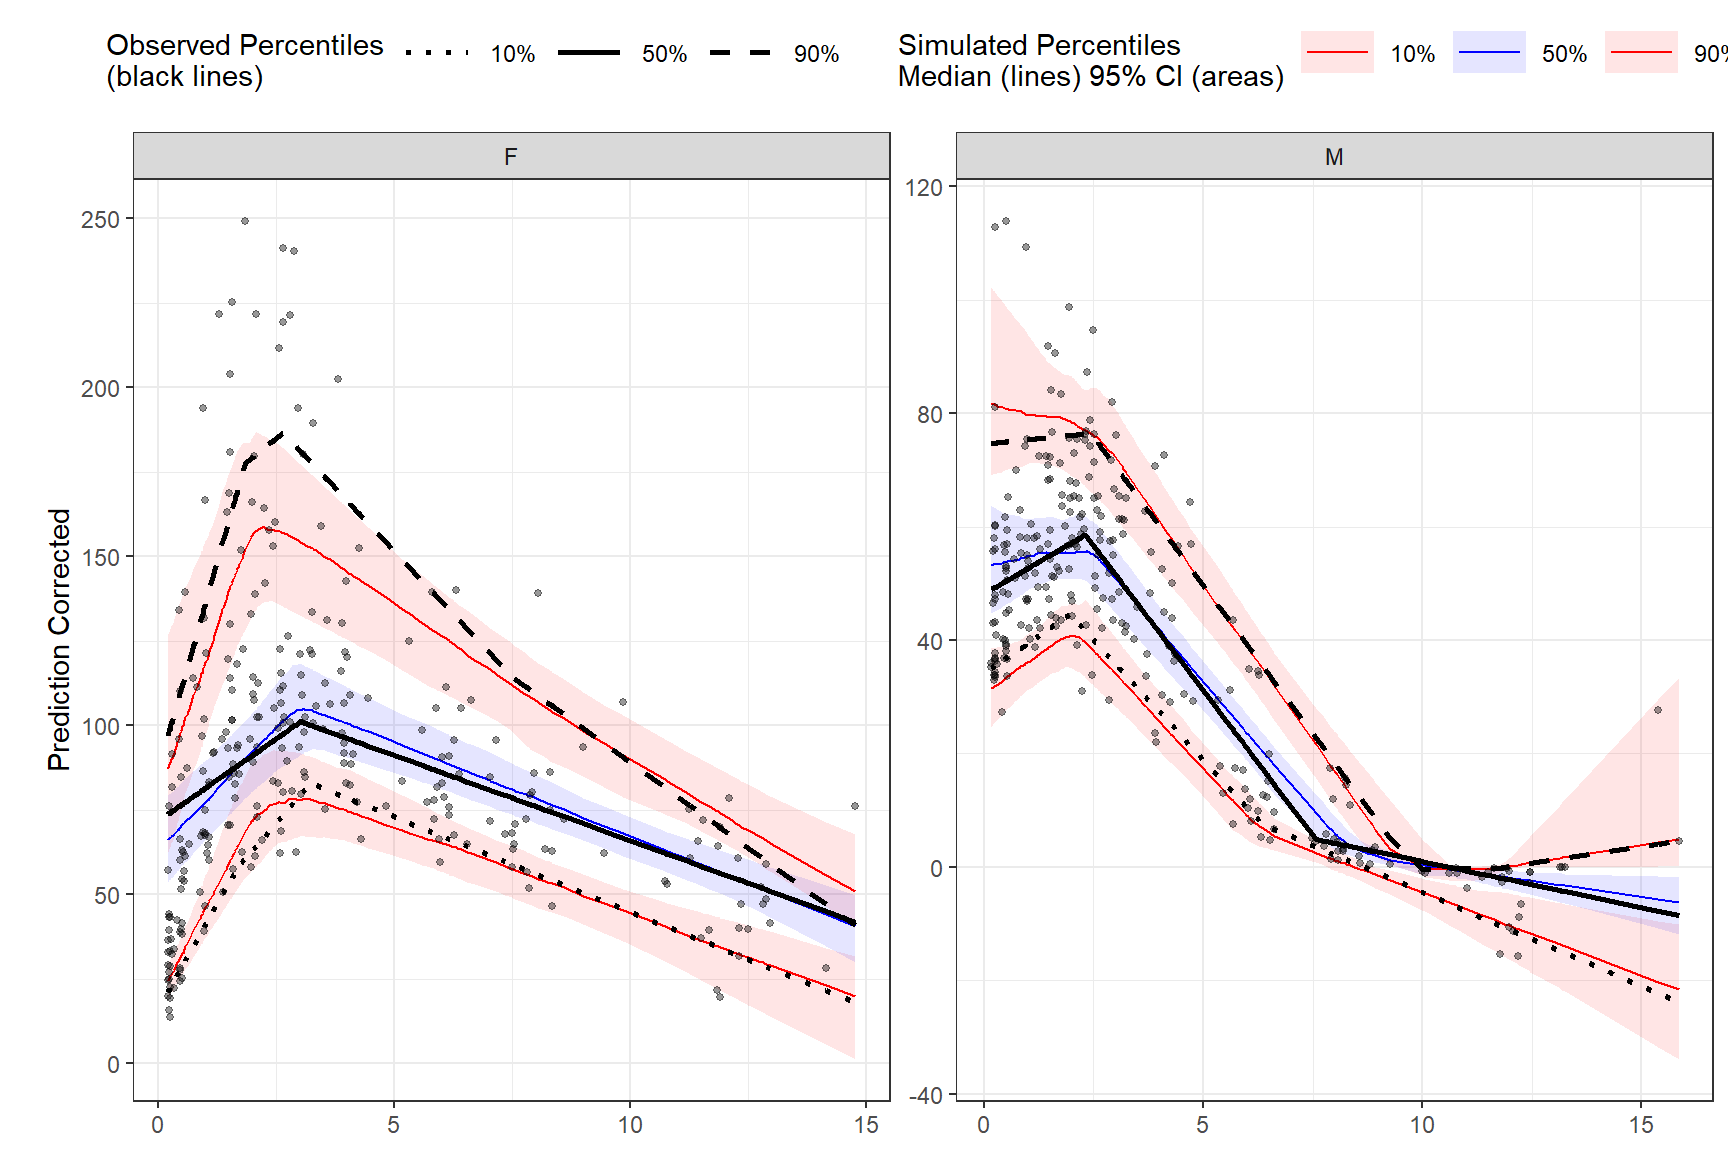
\includegraphics[width=640px]{tidyvpc_bookdown_files/figure-latex/binless-strata-1}

\hypertarget{visualize-bins}{%
\section{Visualize Bins}\label{visualize-bins}}

If using \texttt{binning()} methods, you can visualize bins by using the \texttt{plot()} function on the \texttt{tidyvpcobj} without calling \texttt{vpcstats()}. Once you are satisifed with the binning method, simply call \texttt{vpcstats()} on the existing \texttt{tidyvpcobj} to compute VPC percentiles and prediction intervals i.e \texttt{vpc\ \%\textgreater{}\%\ vpcstats()}

\begin{Shaded}
\begin{Highlighting}[]
\NormalTok{vpc <-}\StringTok{ }\KeywordTok{observed}\NormalTok{(obs_data, }\DataTypeTok{x=}\NormalTok{TIME, }\DataTypeTok{y=}\NormalTok{DV) }\OperatorTok
\StringTok{    }\KeywordTok{simulated}\NormalTok{(sim_data, }\DataTypeTok{y=}\NormalTok{DV) }\OperatorTok
\StringTok{    }\KeywordTok{binning}\NormalTok{(}\DataTypeTok{bin =} \StringTok{"jenks"}\NormalTok{, }\DataTypeTok{nbins =} \DecValTok{7}\NormalTok{)}

\KeywordTok{plot}\NormalTok{(vpc)}
\end{Highlighting}
\end{Shaded}

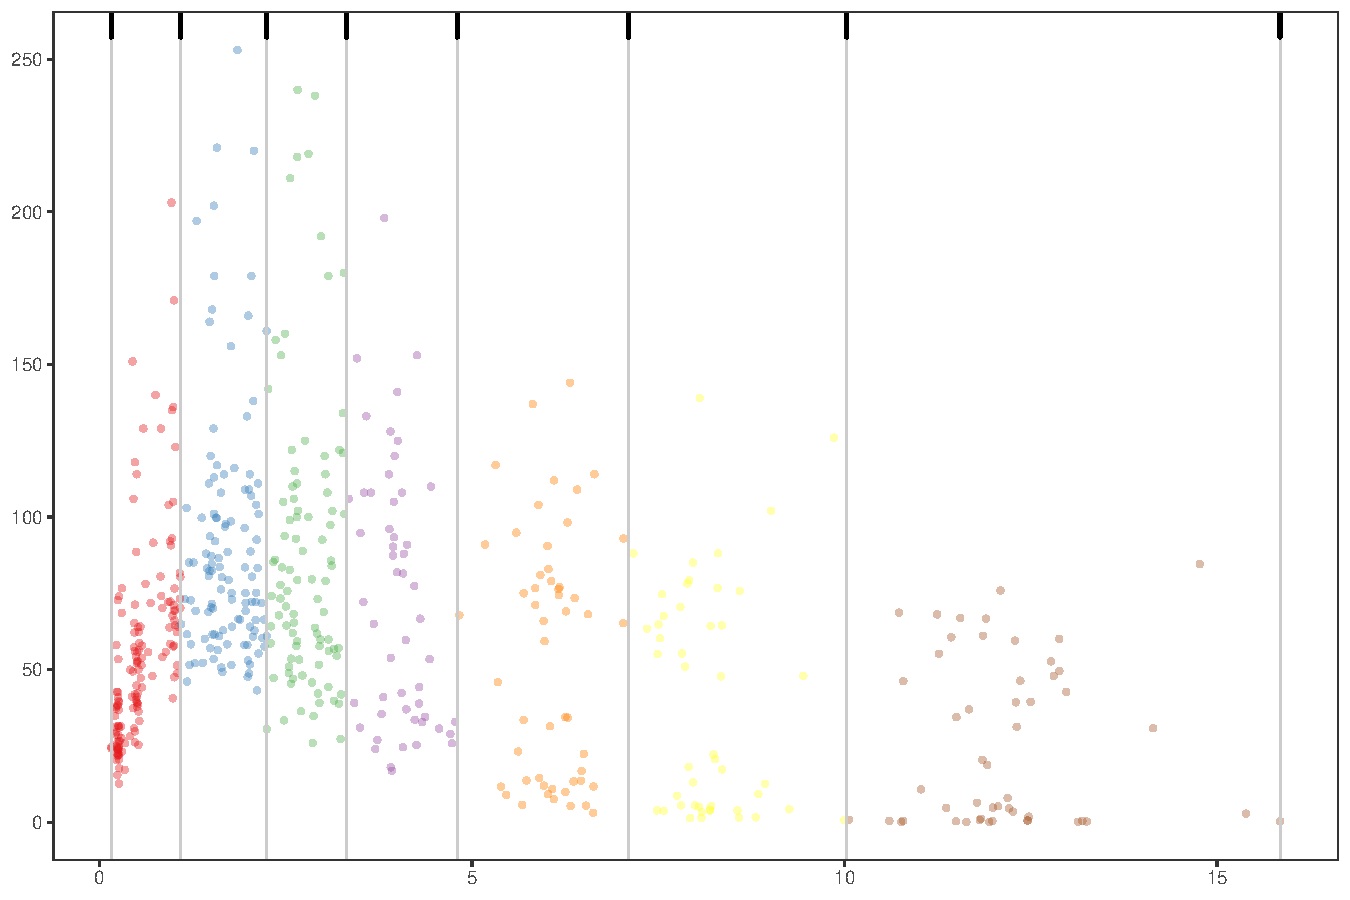
\includegraphics[width=640px]{tidyvpc_bookdown_files/figure-latex/bin-visualize-1}

\hypertarget{bin-information}{%
\section{Bin Information}\label{bin-information}}

To obtain information about the bins, including the number of observations, xmedian, xmean, xmin, xmax, xmidpoint, xleft, xright, and xcenter, use the \texttt{bininfo()} function from \texttt{tidyvpc}.

\begin{Shaded}
\begin{Highlighting}[]
\NormalTok{vpc <-}\StringTok{ }\KeywordTok{observed}\NormalTok{(obs_data, }\DataTypeTok{x=}\NormalTok{TIME, }\DataTypeTok{y=}\NormalTok{DV) }\OperatorTok
\StringTok{    }\KeywordTok{simulated}\NormalTok{(sim_data, }\DataTypeTok{y=}\NormalTok{DV) }\OperatorTok
\StringTok{    }\KeywordTok{binning}\NormalTok{(}\DataTypeTok{bin =} \StringTok{"jenks"}\NormalTok{, }\DataTypeTok{nbins =} \DecValTok{4}\NormalTok{) }\OperatorTok
\StringTok{    }\KeywordTok{vpcstats}\NormalTok{()}

\NormalTok{bin_information <-}\StringTok{ }\KeywordTok{bininfo}\NormalTok{(vpc)}
\KeywordTok{head}\NormalTok{(bin_information)}
\end{Highlighting}
\end{Shaded}

\begin{verbatim}
##             bin nobs    xmedian      xmean      xmin      xmax      xmid
## 1: [0.158,1.89)  213  0.8418133  0.8717959 0.1575342  1.860852  1.009193
## 2:  [1.89,4.83)  187  2.8021930  2.9458444 1.8851078  4.772347  3.328727
## 3:  [4.83,9.45)   96  6.6279698  6.9869973 4.8283449  9.259398  7.043872
## 4:  [9.45,15.8]   54 11.9639045 12.0388598 9.4470340 15.848161 12.647597
##        xleft    xright   xcenter
## 1: 0.1575342  1.872980  1.015257
## 2: 1.8729798  4.800346  3.336663
## 3: 4.8003458  9.353216  7.076781
## 4: 9.3532162 15.848161 12.600688
\end{verbatim}

\hypertarget{ggplot2}{%
\chapter{\texorpdfstring{Extending Further with \texttt{ggplot2}}{Extending Further with ggplot2}}\label{ggplot2}}

While the built in \texttt{plot()} function make it easy to quickly visualize the derived VPC, the \texttt{tidyvpcobj} can be plotted using \texttt{ggplot2} for complete plot customization.

\hypertarget{plot-vpc}{%
\section{Plot VPC}\label{plot-vpc}}

\begin{Shaded}
\begin{Highlighting}[]
\NormalTok{obs_data}\OperatorTok{$}\NormalTok{LLOQ <-}\StringTok{ }\KeywordTok{ifelse}\NormalTok{(obs_data}\OperatorTok{$}\NormalTok{STUDY }\OperatorTok{==}\StringTok{ "Study A"}\NormalTok{, }\DecValTok{50}\NormalTok{, }\DecValTok{25}\NormalTok{)}
\KeywordTok{library}\NormalTok{(dplyr)}

\NormalTok{vpc <-}\StringTok{ }\KeywordTok{observed}\NormalTok{(obs_data, }\DataTypeTok{x =}\NormalTok{ TIME, }\DataTypeTok{y =}\NormalTok{ DV) }\OperatorTok
\StringTok{  }\KeywordTok{simulated}\NormalTok{(sim_data, }\DataTypeTok{y =}\NormalTok{ DV) }\OperatorTok
\StringTok{  }\KeywordTok{censoring}\NormalTok{(}\DataTypeTok{blq =}\NormalTok{ DV }\OperatorTok{<}\StringTok{ }\NormalTok{LLOQ, }\DataTypeTok{lloq =}\NormalTok{ LLOQ) }\OperatorTok
\StringTok{  }\KeywordTok{stratify}\NormalTok{(}\OperatorTok{~}\NormalTok{STUDY) }\OperatorTok
\StringTok{  }\KeywordTok{binning}\NormalTok{(}\DataTypeTok{bin =}\NormalTok{ NTIME) }\OperatorTok
\StringTok{  }\KeywordTok{vpcstats}\NormalTok{(}\DataTypeTok{qpred =} \KeywordTok{c}\NormalTok{(}\FloatTok{0.1}\NormalTok{, }\FloatTok{0.5}\NormalTok{, }\FloatTok{0.9}\NormalTok{))}

\KeywordTok{ggplot}\NormalTok{(vpc}\OperatorTok{$}\NormalTok{stats, }\KeywordTok{aes}\NormalTok{(}\DataTypeTok{x =}\NormalTok{ xbin)) }\OperatorTok{+}\StringTok{ }
\StringTok{  }\KeywordTok{facet_grid}\NormalTok{(}\OperatorTok{~}\NormalTok{STUDY, }\DataTypeTok{scales =} \StringTok{"free"}\NormalTok{, }\DataTypeTok{as.table =} \OtherTok{FALSE}\NormalTok{) }\OperatorTok{+}\StringTok{ }
\StringTok{  }\KeywordTok{geom_ribbon}\NormalTok{(}\KeywordTok{aes}\NormalTok{(}\DataTypeTok{ymin =}\NormalTok{ lo, }\DataTypeTok{ymax =}\NormalTok{ hi, }\DataTypeTok{fill =}\NormalTok{ qname, }\DataTypeTok{col =}\NormalTok{ qname, }\DataTypeTok{group =}\NormalTok{ qname),}\DataTypeTok{alpha =} \FloatTok{0.1}\NormalTok{, }\DataTypeTok{col =} \OtherTok{NA}\NormalTok{) }\OperatorTok{+}\StringTok{ }
\StringTok{  }\KeywordTok{geom_line}\NormalTok{(}\KeywordTok{aes}\NormalTok{(}\DataTypeTok{y =}\NormalTok{ md, }\DataTypeTok{col =}\NormalTok{ qname, }\DataTypeTok{group =}\NormalTok{ qname)) }\OperatorTok{+}
\StringTok{  }\KeywordTok{geom_line}\NormalTok{(}\KeywordTok{aes}\NormalTok{(}\DataTypeTok{y =}\NormalTok{ y, }\DataTypeTok{linetype =}\NormalTok{ qname), }\DataTypeTok{size =} \DecValTok{1}\NormalTok{) }\OperatorTok{+}\StringTok{ }
\StringTok{  }\KeywordTok{geom_hline}\NormalTok{(}\DataTypeTok{data=}\KeywordTok{unique}\NormalTok{(obs_data[, .(STUDY, LLOQ)]), }\KeywordTok{aes}\NormalTok{(}\DataTypeTok{yintercept=}\NormalTok{LLOQ), }\DataTypeTok{linetype=}\StringTok{"dotted"}\NormalTok{, }\DataTypeTok{size=}\DecValTok{1}\NormalTok{) }\OperatorTok{+}
\StringTok{  }\KeywordTok{geom_text}\NormalTok{(}\DataTypeTok{data =} \KeywordTok{unique}\NormalTok{(vpc}\OperatorTok{$}\NormalTok{data[, .(LLOQ), }\DataTypeTok{by =} \StringTok{"STUDY"}\NormalTok{]), }
            \KeywordTok{aes}\NormalTok{(}\DataTypeTok{x =} \DecValTok{10}\NormalTok{, }\DataTypeTok{y =}\NormalTok{ LLOQ, }\DataTypeTok{label =} \KeywordTok{paste}\NormalTok{(}\StringTok{"LLOQ"}\NormalTok{, LLOQ, }\DataTypeTok{sep =} \StringTok{"="}\NormalTok{), ), }\DataTypeTok{vjust =} \DecValTok{1}\NormalTok{, }\DataTypeTok{hjust =} \DecValTok{1}\NormalTok{) }\OperatorTok{+}
\StringTok{  }\KeywordTok{scale_colour_manual}\NormalTok{(}\DataTypeTok{name =} \StringTok{"Simulated Percentiles}\CharTok{\textbackslash{}n}\StringTok{Median (lines) 95% CI (areas)"}\NormalTok{,}
                    \DataTypeTok{breaks =} \KeywordTok{c}\NormalTok{(}\StringTok{"q0.1"}\NormalTok{, }\StringTok{"q0.5"}\NormalTok{, }\StringTok{"q0.9"}\NormalTok{), }
                    \DataTypeTok{values =} \KeywordTok{c}\NormalTok{(}\StringTok{"red"}\NormalTok{, }\StringTok{"blue"}\NormalTok{, }\StringTok{"red"}\NormalTok{), }
                    \DataTypeTok{labels =} \KeywordTok{c}\NormalTok{(}\StringTok{"10%"}\NormalTok{, }\StringTok{"50%"}\NormalTok{, }\StringTok{"90%"}\NormalTok{)) }\OperatorTok{+}\StringTok{ }
\StringTok{  }\KeywordTok{scale_fill_manual}\NormalTok{(}\DataTypeTok{name =} \StringTok{"Simulated Percentiles}\CharTok{\textbackslash{}n}\StringTok{Median (lines) 95% CI (areas)"}\NormalTok{, }
                    \DataTypeTok{breaks =} \KeywordTok{c}\NormalTok{(}\StringTok{"q0.1"}\NormalTok{, }\StringTok{"q0.5"}\NormalTok{, }\StringTok{"q0.9"}\NormalTok{), }
                    \DataTypeTok{values =} \KeywordTok{c}\NormalTok{(}\StringTok{"red"}\NormalTok{, }\StringTok{"blue"}\NormalTok{, }\StringTok{"red"}\NormalTok{), }
                    \DataTypeTok{labels =} \KeywordTok{c}\NormalTok{(}\StringTok{"10%"}\NormalTok{, }\StringTok{"50%"}\NormalTok{, }\StringTok{"90%"}\NormalTok{)) }\OperatorTok{+}\StringTok{ }
\StringTok{  }\KeywordTok{scale_linetype_manual}\NormalTok{(}\DataTypeTok{name =} \StringTok{"Observed Percentiles}\CharTok{\textbackslash{}n}\StringTok{Median (lines) 95% CI (areas)"}\NormalTok{, }
                    \DataTypeTok{breaks =} \KeywordTok{c}\NormalTok{(}\StringTok{"q0.1"}\NormalTok{, }\StringTok{"q0.5"}\NormalTok{, }\StringTok{"q0.9"}\NormalTok{), }
                    \DataTypeTok{values =} \KeywordTok{c}\NormalTok{(}\StringTok{"dotted"}\NormalTok{, }\StringTok{"solid"}\NormalTok{, }\StringTok{"dashed"}\NormalTok{), }
                    \DataTypeTok{labels =} \KeywordTok{c}\NormalTok{(}\StringTok{"10%"}\NormalTok{, }\StringTok{"50%"}\NormalTok{, }\StringTok{"90%"}\NormalTok{)) }\OperatorTok{+}\StringTok{ }
\StringTok{  }\KeywordTok{guides}\NormalTok{(}\DataTypeTok{fill =} \KeywordTok{guide_legend}\NormalTok{(}\DataTypeTok{order =} \DecValTok{2}\NormalTok{), }\DataTypeTok{colour =} \KeywordTok{guide_legend}\NormalTok{(}\DataTypeTok{order =} \DecValTok{2}\NormalTok{), }\DataTypeTok{linetype =} \KeywordTok{guide_legend}\NormalTok{(}\DataTypeTok{order =} \DecValTok{1}\NormalTok{)) }\OperatorTok{+}\StringTok{ }
\StringTok{  }\KeywordTok{theme}\NormalTok{(}\DataTypeTok{legend.position =} \StringTok{"top"}\NormalTok{, }\DataTypeTok{legend.key.width =}\NormalTok{ grid}\OperatorTok{::}\KeywordTok{unit}\NormalTok{(}\DecValTok{1}\NormalTok{, }\StringTok{"cm"}\NormalTok{)) }\OperatorTok{+}\StringTok{ }
\StringTok{  }\KeywordTok{labs}\NormalTok{(}\DataTypeTok{x =} \StringTok{"TIME"}\NormalTok{, }\DataTypeTok{y =} \StringTok{"Concentration"}\NormalTok{) }\OperatorTok{+}\StringTok{ }
\StringTok{  }\KeywordTok{geom_point}\NormalTok{(}\DataTypeTok{data =}\NormalTok{ vpc}\OperatorTok{$}\NormalTok{obs, }\KeywordTok{aes}\NormalTok{(}\DataTypeTok{x =}\NormalTok{ x, }\DataTypeTok{y =}\NormalTok{ y), }\DataTypeTok{size =} \DecValTok{1}\NormalTok{, }\DataTypeTok{alpha =} \FloatTok{0.1}\NormalTok{, }\DataTypeTok{show.legend =} \OtherTok{FALSE}\NormalTok{) }\OperatorTok{+}\StringTok{ }
\StringTok{  }\KeywordTok{geom_vline}\NormalTok{(}\DataTypeTok{data =} \KeywordTok{bininfo}\NormalTok{(vpc)[, .(}\DataTypeTok{x =} \KeywordTok{sort}\NormalTok{(}\KeywordTok{unique}\NormalTok{(}\KeywordTok{c}\NormalTok{(xleft, xright)))), }\DataTypeTok{by =} \KeywordTok{names}\NormalTok{(vpc}\OperatorTok{$}\NormalTok{strat)],}\KeywordTok{aes}\NormalTok{(}\DataTypeTok{xintercept =}\NormalTok{ x), }\DataTypeTok{size =} \KeywordTok{rel}\NormalTok{(}\FloatTok{0.5}\NormalTok{), }\DataTypeTok{col =} \StringTok{"gray80"}\NormalTok{) }\OperatorTok{+}\StringTok{ }
\StringTok{  }\KeywordTok{theme}\NormalTok{(}\DataTypeTok{panel.grid =} \KeywordTok{element_blank}\NormalTok{()) }\OperatorTok{+}\StringTok{ }
\StringTok{  }\KeywordTok{geom_rug}\NormalTok{(}\DataTypeTok{data =} \KeywordTok{bininfo}\NormalTok{(vpc)[, .(}\DataTypeTok{x =} \KeywordTok{sort}\NormalTok{(}\KeywordTok{unique}\NormalTok{(}\KeywordTok{c}\NormalTok{(xleft, xright)))), }\DataTypeTok{by =} \KeywordTok{names}\NormalTok{(vpc}\OperatorTok{$}\NormalTok{strat)],}\KeywordTok{aes}\NormalTok{(}\DataTypeTok{x =}\NormalTok{ x), }\DataTypeTok{sides =} \StringTok{"t"}\NormalTok{, }\DataTypeTok{size =} \DecValTok{1}\NormalTok{)}
\end{Highlighting}
\end{Shaded}

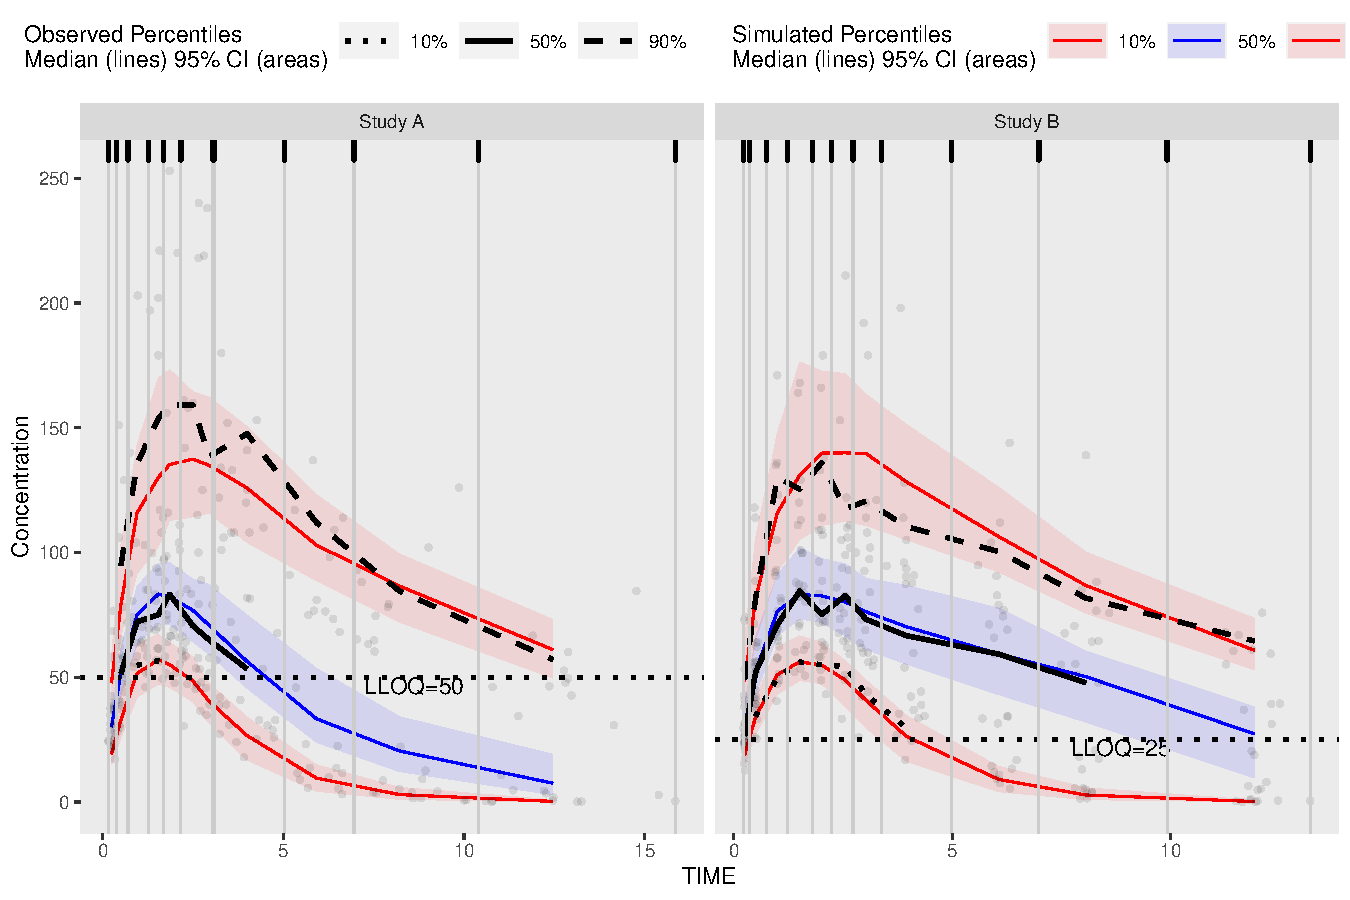
\includegraphics[width=640px]{tidyvpc_bookdown_files/figure-latex/unnamed-chunk-25-1}

\hypertarget{plot-rectangles}{%
\section{Plot Rectangles}\label{plot-rectangles}}

The results from \texttt{bininfo()} make it easy to plot a rectangle VPC using \texttt{ggplot2}.

\begin{Shaded}
\begin{Highlighting}[]
\NormalTok{vpc <-}\StringTok{ }\KeywordTok{observed}\NormalTok{(obs_data, }\DataTypeTok{x=}\NormalTok{TIME, }\DataTypeTok{y=}\NormalTok{DV) }\OperatorTok
\StringTok{    }\KeywordTok{simulated}\NormalTok{(sim_data, }\DataTypeTok{y=}\NormalTok{DV) }\OperatorTok
\StringTok{    }\KeywordTok{binning}\NormalTok{(}\DataTypeTok{bin =} \StringTok{"jenks"}\NormalTok{, }\DataTypeTok{nbins =} \DecValTok{4}\NormalTok{) }\OperatorTok
\StringTok{    }\KeywordTok{vpcstats}\NormalTok{()}

\CommentTok{#Get vpcstats df}
\NormalTok{stats <-}\StringTok{ }\NormalTok{vpc}\OperatorTok{$}\NormalTok{stats}
\CommentTok{#Get bininfo df}
\NormalTok{bin_information <-}\StringTok{ }\KeywordTok{bininfo}\NormalTok{(vpc)}
\CommentTok{#Left join bin_info to vpcstats on bin}
\NormalTok{bin_information <-}\StringTok{ }\NormalTok{stats[bin_information, on =}\StringTok{ "bin"}\NormalTok{]}
\CommentTok{#Generate ymin}
\NormalTok{bin_information <-}\StringTok{ }\NormalTok{bin_information[, ymin }\OperatorTok{:}\ErrorTok{=}\StringTok{ }\KeywordTok{min}\NormalTok{(y), by =}\StringTok{ "bin"}\NormalTok{]}
\CommentTok{#Generate ymax}
\NormalTok{bin_information <-}\StringTok{ }\NormalTok{bin_information[, ymax }\OperatorTok{:}\ErrorTok{=}\StringTok{ }\KeywordTok{max}\NormalTok{(y), by =}\StringTok{ "bin"}\NormalTok{]}
\KeywordTok{head}\NormalTok{(bin_information)}
\end{Highlighting}
\end{Shaded}

\begin{verbatim}
##             bin      xbin qname      y        lo       md        hi nobs
## 1: [0.158,1.89) 0.8418133 q0.05  22.94  19.05306  22.1295  26.32546  213
## 2: [0.158,1.89) 0.8418133  q0.5  61.50  56.61835  61.7225  68.59207  213
## 3: [0.158,1.89) 0.8418133 q0.95 144.40 108.56340 132.0360 156.84105  213
## 4:  [1.89,4.83) 2.8021930 q0.05  29.38  23.01417  28.2300  32.95001  187
## 5:  [1.89,4.83) 2.8021930  q0.5  74.10  66.70315  75.9475  82.94110  187
## 6:  [1.89,4.83) 2.8021930 q0.95 179.00 135.74530 155.3395 180.72525  187
##      xmedian     xmean      xmin     xmax     xmid     xleft   xright  xcenter
## 1: 0.8418133 0.8717959 0.1575342 1.860852 1.009193 0.1575342 1.872980 1.015257
## 2: 0.8418133 0.8717959 0.1575342 1.860852 1.009193 0.1575342 1.872980 1.015257
## 3: 0.8418133 0.8717959 0.1575342 1.860852 1.009193 0.1575342 1.872980 1.015257
## 4: 2.8021930 2.9458444 1.8851078 4.772347 3.328727 1.8729798 4.800346 3.336663
## 5: 2.8021930 2.9458444 1.8851078 4.772347 3.328727 1.8729798 4.800346 3.336663
## 6: 2.8021930 2.9458444 1.8851078 4.772347 3.328727 1.8729798 4.800346 3.336663
##     ymin  ymax
## 1: 22.94 144.4
## 2: 22.94 144.4
## 3: 22.94 144.4
## 4: 29.38 179.0
## 5: 29.38 179.0
## 6: 29.38 179.0
\end{verbatim}

Plot rectangles using \texttt{ymin} and \texttt{ymax}, the min/max y values in \texttt{vpc\$stats} grouped by bin.

\begin{Shaded}
\begin{Highlighting}[]
\KeywordTok{ggplot}\NormalTok{(bin_information, }\KeywordTok{aes}\NormalTok{(}\DataTypeTok{x =}\NormalTok{ xbin)) }\OperatorTok{+}\StringTok{ }
\StringTok{  }\KeywordTok{geom_line}\NormalTok{(}\KeywordTok{aes}\NormalTok{(}\DataTypeTok{y =}\NormalTok{ md, }\DataTypeTok{col =}\NormalTok{ qname, }\DataTypeTok{group =}\NormalTok{ qname)) }\OperatorTok{+}
\StringTok{  }\KeywordTok{geom_line}\NormalTok{(}\KeywordTok{aes}\NormalTok{(}\DataTypeTok{y =}\NormalTok{ y, }\DataTypeTok{linetype =}\NormalTok{ qname), }\DataTypeTok{size =} \DecValTok{1}\NormalTok{) }\OperatorTok{+}
\StringTok{  }\KeywordTok{geom_rect}\NormalTok{(}\KeywordTok{aes}\NormalTok{(}\DataTypeTok{xmin=}\NormalTok{ xleft,}\DataTypeTok{xmax=}\NormalTok{ xright, }\DataTypeTok{ymin =}\NormalTok{  ymin, }\DataTypeTok{ymax =}\NormalTok{  ymax),}\DataTypeTok{alpha =} \FloatTok{.1}\NormalTok{, }\DataTypeTok{col =} \StringTok{"black"}\NormalTok{, }\DataTypeTok{fill =} \StringTok{"green"}\NormalTok{) }\OperatorTok{+}
\StringTok{  }\KeywordTok{geom_point}\NormalTok{(}\DataTypeTok{data =}\NormalTok{ vpc}\OperatorTok{$}\NormalTok{obs, }\KeywordTok{aes}\NormalTok{(}\DataTypeTok{x =}\NormalTok{ x, }\DataTypeTok{y =}\NormalTok{ y), }\DataTypeTok{size =} \DecValTok{1}\NormalTok{, }\DataTypeTok{alpha =} \FloatTok{0.1}\NormalTok{, }\DataTypeTok{show.legend =} \OtherTok{FALSE}\NormalTok{) }\OperatorTok{+}\StringTok{ }
\StringTok{  }\KeywordTok{scale_colour_manual}\NormalTok{(}\DataTypeTok{name =} \StringTok{"Simulated Percentiles}\CharTok{\textbackslash{}n}\StringTok{Median (lines) 95% CI (areas)"}\NormalTok{,}
                    \DataTypeTok{breaks =} \KeywordTok{c}\NormalTok{(}\StringTok{"q0.05"}\NormalTok{, }\StringTok{"q0.5"}\NormalTok{, }\StringTok{"q0.95"}\NormalTok{), }
                    \DataTypeTok{values =} \KeywordTok{c}\NormalTok{(}\StringTok{"red"}\NormalTok{, }\StringTok{"blue"}\NormalTok{, }\StringTok{"red"}\NormalTok{), }
                    \DataTypeTok{labels =} \KeywordTok{c}\NormalTok{(}\StringTok{"5%"}\NormalTok{, }\StringTok{"50%"}\NormalTok{, }\StringTok{"95%"}\NormalTok{)) }\OperatorTok{+}\StringTok{ }
\StringTok{  }\KeywordTok{scale_linetype_manual}\NormalTok{(}\DataTypeTok{name =} \StringTok{"Observed Percentiles}\CharTok{\textbackslash{}n}\StringTok{Median (lines) 95% CI (areas)"}\NormalTok{, }
                    \DataTypeTok{breaks =} \KeywordTok{c}\NormalTok{(}\StringTok{"q0.05"}\NormalTok{, }\StringTok{"q0.5"}\NormalTok{, }\StringTok{"q0.95"}\NormalTok{), }
                    \DataTypeTok{values =} \KeywordTok{c}\NormalTok{(}\StringTok{"dotted"}\NormalTok{, }\StringTok{"solid"}\NormalTok{, }\StringTok{"dashed"}\NormalTok{), }
                    \DataTypeTok{labels =} \KeywordTok{c}\NormalTok{(}\StringTok{"5%"}\NormalTok{, }\StringTok{"50%"}\NormalTok{, }\StringTok{"95%"}\NormalTok{)) }\OperatorTok{+}\StringTok{ }
\StringTok{  }\KeywordTok{geom_vline}\NormalTok{(}\DataTypeTok{data =}\NormalTok{ bin_information[, }\KeywordTok{list}\NormalTok{(}\DataTypeTok{x =} \KeywordTok{sort}\NormalTok{(}\KeywordTok{unique}\NormalTok{(}\KeywordTok{c}\NormalTok{(xleft, xright))))],}\KeywordTok{aes}\NormalTok{(}\DataTypeTok{xintercept =}\NormalTok{ x), }\DataTypeTok{size =} \KeywordTok{rel}\NormalTok{(}\FloatTok{0.5}\NormalTok{), }\DataTypeTok{col =} \StringTok{"gray80"}\NormalTok{) }\OperatorTok{+}
\StringTok{  }\KeywordTok{geom_rug}\NormalTok{(}\DataTypeTok{data =}\NormalTok{ bin_information[, }\KeywordTok{list}\NormalTok{(}\DataTypeTok{x =} \KeywordTok{sort}\NormalTok{(}\KeywordTok{unique}\NormalTok{(}\KeywordTok{c}\NormalTok{(xleft, xright))))],}\KeywordTok{aes}\NormalTok{(}\DataTypeTok{x =}\NormalTok{ x), }\DataTypeTok{sides =} \StringTok{"t"}\NormalTok{, }\DataTypeTok{size =} \DecValTok{1}\NormalTok{) }\OperatorTok{+}
\StringTok{  }\KeywordTok{guides}\NormalTok{(}\DataTypeTok{fill =} \KeywordTok{guide_legend}\NormalTok{(}\DataTypeTok{order =} \DecValTok{2}\NormalTok{), }\DataTypeTok{colour =} \KeywordTok{guide_legend}\NormalTok{(}\DataTypeTok{order =} \DecValTok{2}\NormalTok{), }\DataTypeTok{linetype =} \KeywordTok{guide_legend}\NormalTok{(}\DataTypeTok{order =} \DecValTok{1}\NormalTok{)) }\OperatorTok{+}\StringTok{ }
\StringTok{  }\KeywordTok{theme}\NormalTok{(}\DataTypeTok{legend.position =} \StringTok{"top"}\NormalTok{, }\DataTypeTok{legend.key.width =}\NormalTok{ grid}\OperatorTok{::}\KeywordTok{unit}\NormalTok{(}\DecValTok{1}\NormalTok{, }\StringTok{"cm"}\NormalTok{)) }\OperatorTok{+}\StringTok{ }
\StringTok{  }\KeywordTok{labs}\NormalTok{(}\DataTypeTok{x =} \StringTok{"TIME"}\NormalTok{, }\DataTypeTok{y =} \StringTok{"Concentration"}\NormalTok{)}
\end{Highlighting}
\end{Shaded}

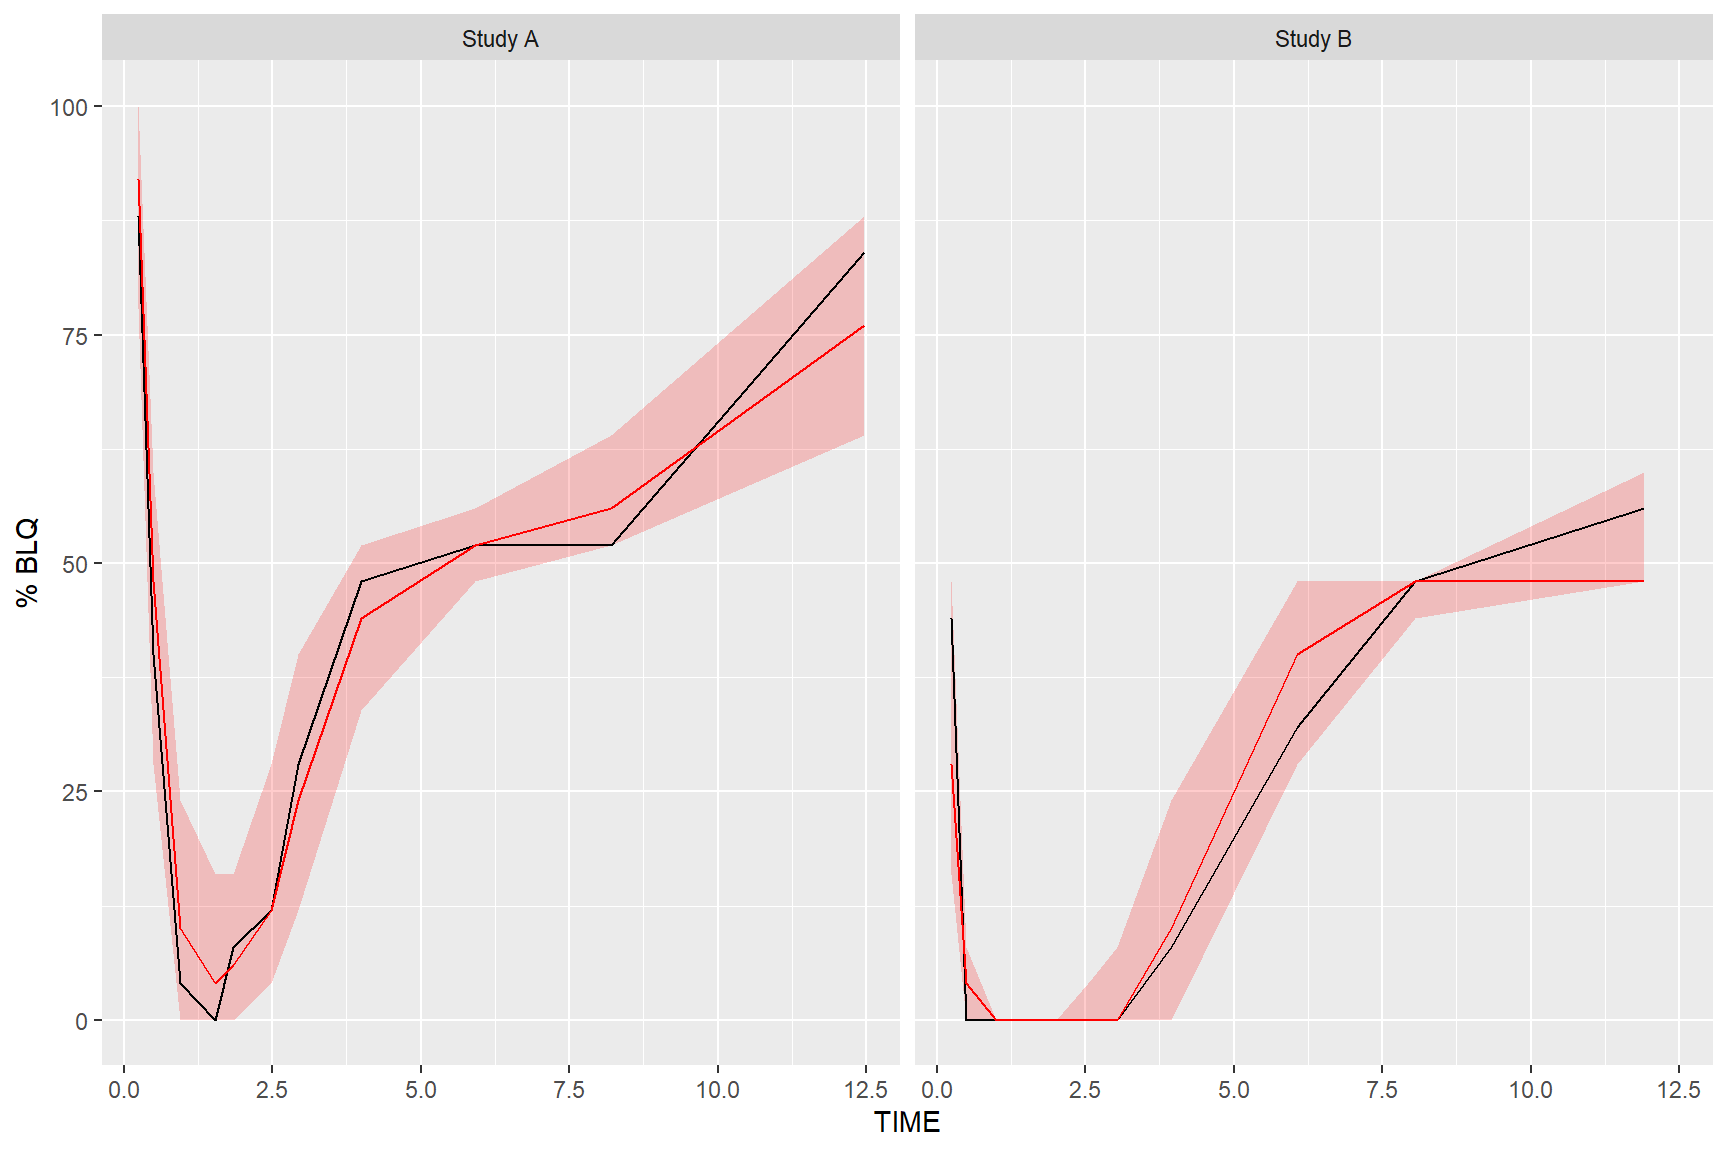
\includegraphics[width=640px]{tidyvpc_bookdown_files/figure-latex/unnamed-chunk-27-1}

Alternatively, we can obtain the required data for plotting used in the above \texttt{bin\_information} data frame by merging \texttt{vpc\$stats} and \texttt{bininfo(vpc)} on \texttt{bin} in the \texttt{ggplot2} data argument. If stratifying you will need to include the name of the stratification variable(s) in the \texttt{data.table} merge i.e.~\texttt{vpc\$stats{[}bininfo(vpc),\ on=c("STUDY",\ "bin"){]}}. In the rectangle vpc below, we will stratify on \texttt{STUDY} and plot rectangles for each quantile.

\begin{Shaded}
\begin{Highlighting}[]
\NormalTok{obs_data}\OperatorTok{$}\NormalTok{LLOQ <-}\StringTok{ }\NormalTok{obs_data[, }\KeywordTok{ifelse}\NormalTok{(STUDY }\OperatorTok{==}\StringTok{ "Study A"}\NormalTok{, }\DecValTok{50}\NormalTok{, }\DecValTok{25}\NormalTok{)]}

\NormalTok{vpc <-}\StringTok{ }\KeywordTok{observed}\NormalTok{(obs_data, }\DataTypeTok{x =}\NormalTok{ TIME, }\DataTypeTok{y =}\NormalTok{ DV) }\OperatorTok
\StringTok{  }\KeywordTok{simulated}\NormalTok{(sim_data, }\DataTypeTok{y =}\NormalTok{ DV) }\OperatorTok
\StringTok{  }\KeywordTok{censoring}\NormalTok{(}\DataTypeTok{blq =}\NormalTok{ DV }\OperatorTok{<}\StringTok{ }\NormalTok{LLOQ, }\DataTypeTok{lloq =}\NormalTok{ LLOQ) }\OperatorTok
\StringTok{  }\KeywordTok{stratify}\NormalTok{(}\OperatorTok{~}\NormalTok{STUDY) }\OperatorTok
\StringTok{  }\KeywordTok{binning}\NormalTok{(}\DataTypeTok{bin =}\NormalTok{ NTIME) }\OperatorTok
\StringTok{  }\KeywordTok{vpcstats}\NormalTok{(}\DataTypeTok{qpred =} \KeywordTok{c}\NormalTok{(}\FloatTok{0.1}\NormalTok{, }\FloatTok{0.5}\NormalTok{, }\FloatTok{0.9}\NormalTok{))}


\KeywordTok{ggplot}\NormalTok{(vpc}\OperatorTok{$}\NormalTok{stats[}\KeywordTok{bininfo}\NormalTok{(vpc), }\DataTypeTok{on=}\KeywordTok{c}\NormalTok{(}\StringTok{"STUDY"}\NormalTok{, }\StringTok{"bin"}\NormalTok{)], }\KeywordTok{aes}\NormalTok{(}\DataTypeTok{x =}\NormalTok{ xbin)) }\OperatorTok{+}\StringTok{ }
\StringTok{  }\KeywordTok{facet_grid}\NormalTok{(}\OperatorTok{~}\NormalTok{STUDY, }\DataTypeTok{scales =} \StringTok{"free"}\NormalTok{, }\DataTypeTok{as.table =} \OtherTok{FALSE}\NormalTok{) }\OperatorTok{+}\StringTok{ }
\StringTok{  }\KeywordTok{geom_rect}\NormalTok{(}\KeywordTok{aes}\NormalTok{(}\DataTypeTok{xmin =}\NormalTok{ xleft, }\DataTypeTok{xmax =}\NormalTok{ xright, }\DataTypeTok{ymin =}\NormalTok{ lo, }\DataTypeTok{ymax =}\NormalTok{ hi, }\DataTypeTok{fill =}\NormalTok{ qname, }\DataTypeTok{col =}\NormalTok{ qname, }\DataTypeTok{group =}\NormalTok{ qname),}\DataTypeTok{alpha =} \FloatTok{0.1}\NormalTok{, }\DataTypeTok{col =} \OtherTok{NA}\NormalTok{) }\OperatorTok{+}\StringTok{ }
\StringTok{  }\KeywordTok{geom_segment}\NormalTok{(}\KeywordTok{aes}\NormalTok{(}\DataTypeTok{x =}\NormalTok{ xleft, }\DataTypeTok{xend =}\NormalTok{ xright, }\DataTypeTok{y =}\NormalTok{ md, }\DataTypeTok{yend =}\NormalTok{ md, }\DataTypeTok{col =}\NormalTok{ qname, }\DataTypeTok{group =}\NormalTok{ qname)) }\OperatorTok{+}
\StringTok{  }\KeywordTok{geom_segment}\NormalTok{(}\KeywordTok{aes}\NormalTok{(}\DataTypeTok{x =}\NormalTok{ xleft, }\DataTypeTok{xend =}\NormalTok{ xright, }\DataTypeTok{y =}\NormalTok{ y, }\DataTypeTok{yend =}\NormalTok{ y, }\DataTypeTok{linetype =}\NormalTok{ qname), }\DataTypeTok{size =} \DecValTok{1}\NormalTok{) }\OperatorTok{+}
\StringTok{  }\KeywordTok{geom_line}\NormalTok{(}\KeywordTok{aes}\NormalTok{(}\DataTypeTok{y =}\NormalTok{ md, }\DataTypeTok{col =}\NormalTok{ qname, }\DataTypeTok{group =}\NormalTok{ qname)) }\OperatorTok{+}
\StringTok{  }\KeywordTok{geom_line}\NormalTok{(}\KeywordTok{aes}\NormalTok{(}\DataTypeTok{y =}\NormalTok{ y, }\DataTypeTok{linetype =}\NormalTok{ qname), }\DataTypeTok{size =} \DecValTok{1}\NormalTok{) }\OperatorTok{+}\StringTok{ }
\StringTok{  }\KeywordTok{geom_hline}\NormalTok{(}\DataTypeTok{data=}\KeywordTok{unique}\NormalTok{(obs_data[, }\KeywordTok{list}\NormalTok{(STUDY, LLOQ)]), }\KeywordTok{aes}\NormalTok{(}\DataTypeTok{yintercept=}\NormalTok{LLOQ), }\DataTypeTok{linetype=}\StringTok{"dotted"}\NormalTok{, }\DataTypeTok{size=}\DecValTok{1}\NormalTok{) }\OperatorTok{+}
\StringTok{  }\KeywordTok{geom_text}\NormalTok{(}\DataTypeTok{data =} \KeywordTok{unique}\NormalTok{(vpc}\OperatorTok{$}\NormalTok{data[, }\KeywordTok{list}\NormalTok{(LLOQ), }\DataTypeTok{by =} \StringTok{"STUDY"}\NormalTok{]), }
            \KeywordTok{aes}\NormalTok{(}\DataTypeTok{x =} \DecValTok{10}\NormalTok{, }\DataTypeTok{y =}\NormalTok{ LLOQ, }\DataTypeTok{label =} \KeywordTok{paste}\NormalTok{(}\StringTok{"LLOQ"}\NormalTok{, LLOQ, }\DataTypeTok{sep =} \StringTok{"="}\NormalTok{), ), }\DataTypeTok{vjust =} \DecValTok{1}\NormalTok{, }\DataTypeTok{hjust =} \DecValTok{1}\NormalTok{) }\OperatorTok{+}
\StringTok{  }\KeywordTok{scale_colour_manual}\NormalTok{(}\DataTypeTok{name =} \StringTok{"Simulated Percentiles}\CharTok{\textbackslash{}n}\StringTok{Median (lines) 95% CI (areas)"}\NormalTok{,}
                      \DataTypeTok{breaks =} \KeywordTok{c}\NormalTok{(}\StringTok{"q0.1"}\NormalTok{, }\StringTok{"q0.5"}\NormalTok{, }\StringTok{"q0.9"}\NormalTok{), }
                      \DataTypeTok{values =} \KeywordTok{c}\NormalTok{(}\StringTok{"red"}\NormalTok{, }\StringTok{"blue"}\NormalTok{, }\StringTok{"red"}\NormalTok{), }
                      \DataTypeTok{labels =} \KeywordTok{c}\NormalTok{(}\StringTok{"10%"}\NormalTok{, }\StringTok{"50%"}\NormalTok{, }\StringTok{"90%"}\NormalTok{)) }\OperatorTok{+}\StringTok{ }
\StringTok{  }\KeywordTok{scale_fill_manual}\NormalTok{(}\DataTypeTok{name =} \StringTok{"Simulated Percentiles}\CharTok{\textbackslash{}n}\StringTok{Median (lines) 95% CI (areas)"}\NormalTok{, }
                    \DataTypeTok{breaks =} \KeywordTok{c}\NormalTok{(}\StringTok{"q0.1"}\NormalTok{, }\StringTok{"q0.5"}\NormalTok{, }\StringTok{"q0.9"}\NormalTok{), }
                    \DataTypeTok{values =} \KeywordTok{c}\NormalTok{(}\StringTok{"red"}\NormalTok{, }\StringTok{"blue"}\NormalTok{, }\StringTok{"red"}\NormalTok{), }
                    \DataTypeTok{labels =} \KeywordTok{c}\NormalTok{(}\StringTok{"10%"}\NormalTok{, }\StringTok{"50%"}\NormalTok{, }\StringTok{"90%"}\NormalTok{)) }\OperatorTok{+}\StringTok{ }
\StringTok{  }\KeywordTok{scale_linetype_manual}\NormalTok{(}\DataTypeTok{name =} \StringTok{"Observed Percentiles}\CharTok{\textbackslash{}n}\StringTok{Median (lines) 95% CI (areas)"}\NormalTok{, }
                        \DataTypeTok{breaks =} \KeywordTok{c}\NormalTok{(}\StringTok{"q0.1"}\NormalTok{, }\StringTok{"q0.5"}\NormalTok{, }\StringTok{"q0.9"}\NormalTok{), }
                        \DataTypeTok{values =} \KeywordTok{c}\NormalTok{(}\StringTok{"dotted"}\NormalTok{, }\StringTok{"solid"}\NormalTok{, }\StringTok{"dashed"}\NormalTok{), }
                        \DataTypeTok{labels =} \KeywordTok{c}\NormalTok{(}\StringTok{"10%"}\NormalTok{, }\StringTok{"50%"}\NormalTok{, }\StringTok{"90%"}\NormalTok{)) }\OperatorTok{+}\StringTok{ }
\StringTok{  }\KeywordTok{guides}\NormalTok{(}\DataTypeTok{fill =} \KeywordTok{guide_legend}\NormalTok{(}\DataTypeTok{order =} \DecValTok{2}\NormalTok{), }\DataTypeTok{colour =} \KeywordTok{guide_legend}\NormalTok{(}\DataTypeTok{order =} \DecValTok{2}\NormalTok{), }\DataTypeTok{linetype =} \KeywordTok{guide_legend}\NormalTok{(}\DataTypeTok{order =} \DecValTok{1}\NormalTok{)) }\OperatorTok{+}\StringTok{ }
\StringTok{  }\KeywordTok{theme}\NormalTok{(}\DataTypeTok{legend.position =} \StringTok{"top"}\NormalTok{, }\DataTypeTok{legend.key.width =}\NormalTok{ grid}\OperatorTok{::}\KeywordTok{unit}\NormalTok{(}\DecValTok{1}\NormalTok{, }\StringTok{"cm"}\NormalTok{)) }\OperatorTok{+}\StringTok{ }
\StringTok{  }\KeywordTok{labs}\NormalTok{(}\DataTypeTok{x =} \StringTok{"TIME"}\NormalTok{, }\DataTypeTok{y =} \StringTok{"Concentration"}\NormalTok{) }\OperatorTok{+}\StringTok{ }
\StringTok{  }\KeywordTok{geom_point}\NormalTok{(}\DataTypeTok{data =}\NormalTok{ vpc}\OperatorTok{$}\NormalTok{obs, }\KeywordTok{aes}\NormalTok{(}\DataTypeTok{x =}\NormalTok{ x, }\DataTypeTok{y =}\NormalTok{ y), }\DataTypeTok{size =} \DecValTok{1}\NormalTok{, }\DataTypeTok{alpha =} \FloatTok{0.1}\NormalTok{, }\DataTypeTok{show.legend =} \OtherTok{FALSE}\NormalTok{) }\OperatorTok{+}\StringTok{ }
\StringTok{  }\KeywordTok{geom_vline}\NormalTok{(}\DataTypeTok{data =} \KeywordTok{bininfo}\NormalTok{(vpc)[, }\KeywordTok{list}\NormalTok{(}\DataTypeTok{x =} \KeywordTok{sort}\NormalTok{(}\KeywordTok{unique}\NormalTok{(}\KeywordTok{c}\NormalTok{(xleft, xright)))), }\DataTypeTok{by =} \KeywordTok{names}\NormalTok{(vpc}\OperatorTok{$}\NormalTok{strat)],}\KeywordTok{aes}\NormalTok{(}\DataTypeTok{xintercept =}\NormalTok{ x), }\DataTypeTok{size =} \KeywordTok{rel}\NormalTok{(}\FloatTok{0.5}\NormalTok{), }\DataTypeTok{col =} \StringTok{"gray80"}\NormalTok{) }\OperatorTok{+}\StringTok{ }
\StringTok{  }\KeywordTok{theme}\NormalTok{(}\DataTypeTok{panel.grid =} \KeywordTok{element_blank}\NormalTok{()) }\OperatorTok{+}\StringTok{ }
\StringTok{  }\KeywordTok{geom_rug}\NormalTok{(}\DataTypeTok{data =} \KeywordTok{bininfo}\NormalTok{(vpc)[, }\KeywordTok{list}\NormalTok{(}\DataTypeTok{x =} \KeywordTok{sort}\NormalTok{(}\KeywordTok{unique}\NormalTok{(}\KeywordTok{c}\NormalTok{(xleft, xright)))), }\DataTypeTok{by =} \KeywordTok{names}\NormalTok{(vpc}\OperatorTok{$}\NormalTok{strat)],}\KeywordTok{aes}\NormalTok{(}\DataTypeTok{x =}\NormalTok{ x), }\DataTypeTok{sides =} \StringTok{"t"}\NormalTok{, }\DataTypeTok{size =} \DecValTok{1}\NormalTok{)}
\end{Highlighting}
\end{Shaded}

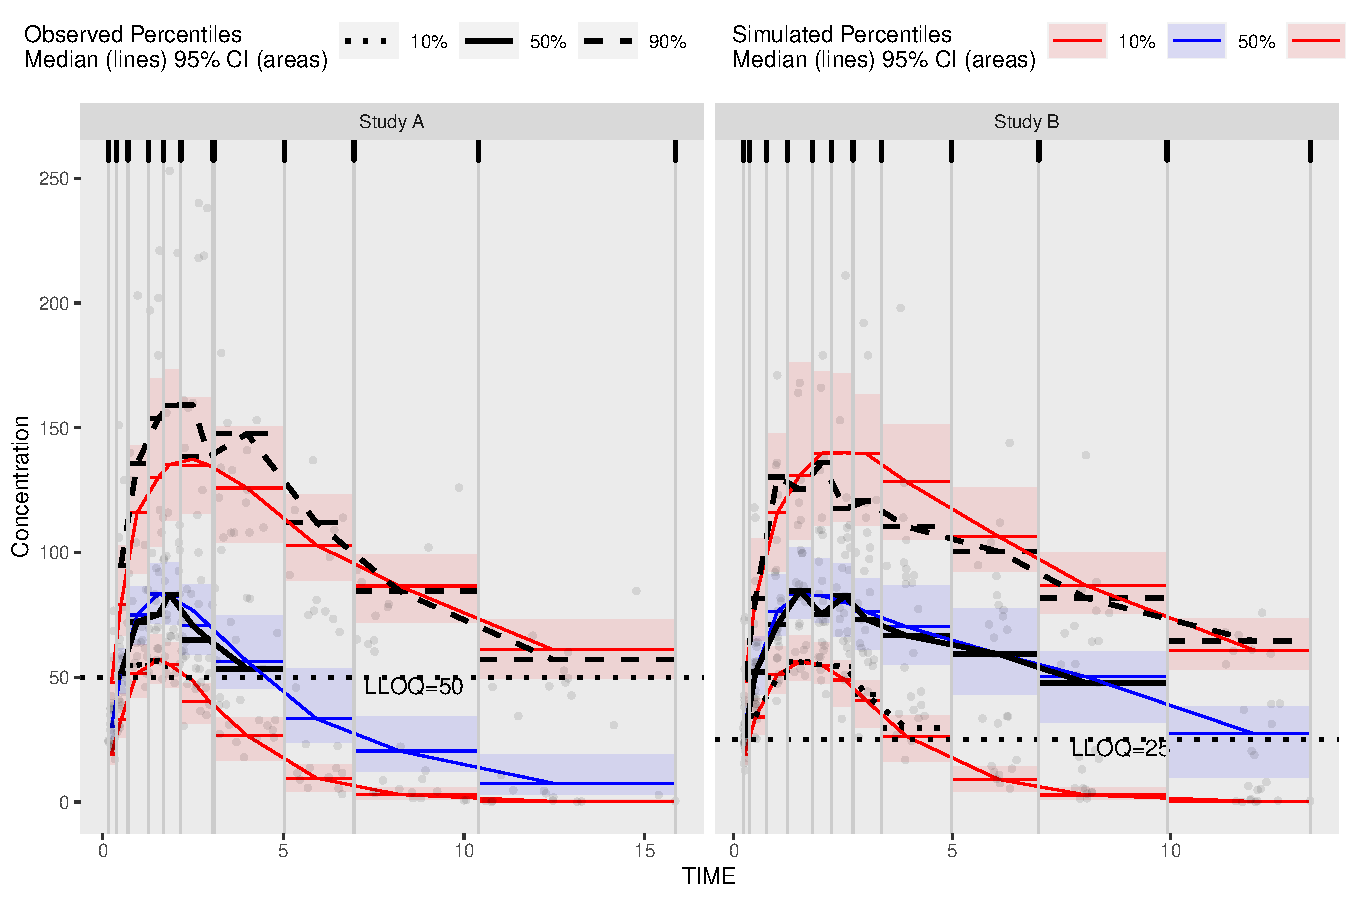
\includegraphics[width=640px]{tidyvpc_bookdown_files/figure-latex/unnamed-chunk-28-1}

\hypertarget{plot-below-quantification-limit-bql}{%
\section{Plot Below Quantification Limit (BQL)}\label{plot-below-quantification-limit-bql}}

If using the \texttt{censoring()} function, the resulting \texttt{tidyvpcobj} will also contain a pctblq table. Use \texttt{ggplot2} to plot the percentage of data below the limit of quantification across bins.

We can include \texttt{geom\_ribbon()} using the \texttt{lo} and \texttt{hi} columns in the \texttt{vpc\$pctblq} table to denote the lower/upper bounds of our confidence interval. Let's also plot the median \%blq of the simulated data using the \texttt{md} column in the \texttt{vpc\$pctblq} table.

\begin{Shaded}
\begin{Highlighting}[]
\NormalTok{obs_data}\OperatorTok{$}\NormalTok{LLOQ <-}\StringTok{ }\KeywordTok{ifelse}\NormalTok{(obs_data}\OperatorTok{$}\NormalTok{STUDY }\OperatorTok{==}\StringTok{ "Study A"}\NormalTok{, }\DecValTok{50}\NormalTok{, }\DecValTok{25}\NormalTok{)}

\NormalTok{vpc <-}\StringTok{ }\KeywordTok{observed}\NormalTok{(obs_data, }\DataTypeTok{x =}\NormalTok{ TIME, }\DataTypeTok{y =}\NormalTok{ DV) }\OperatorTok
\StringTok{  }\KeywordTok{simulated}\NormalTok{(sim_data, }\DataTypeTok{y =}\NormalTok{ DV) }\OperatorTok
\StringTok{  }\KeywordTok{censoring}\NormalTok{(}\DataTypeTok{blq =}\NormalTok{ DV }\OperatorTok{<}\StringTok{ }\NormalTok{LLOQ, }\DataTypeTok{lloq =}\NormalTok{ LLOQ) }\OperatorTok
\StringTok{  }\KeywordTok{stratify}\NormalTok{(}\OperatorTok{~}\NormalTok{STUDY) }\OperatorTok
\StringTok{  }\KeywordTok{binning}\NormalTok{(}\DataTypeTok{bin =}\NormalTok{ NTIME) }\OperatorTok
\StringTok{  }\KeywordTok{vpcstats}\NormalTok{(}\DataTypeTok{qpred =} \KeywordTok{c}\NormalTok{(}\FloatTok{0.1}\NormalTok{, }\FloatTok{0.5}\NormalTok{, }\FloatTok{0.9}\NormalTok{))}

\KeywordTok{ggplot}\NormalTok{(vpc}\OperatorTok{$}\NormalTok{pctblq) }\OperatorTok{+}\StringTok{ }
\StringTok{  }\KeywordTok{facet_grid}\NormalTok{(}\OperatorTok{~}\NormalTok{STUDY) }\OperatorTok{+}
\StringTok{  }\KeywordTok{geom_ribbon}\NormalTok{(}\KeywordTok{aes}\NormalTok{(}\DataTypeTok{x =}\NormalTok{ xbin, }\DataTypeTok{ymin=}\NormalTok{ lo, }\DataTypeTok{ymax =}\NormalTok{ hi), }\DataTypeTok{fill =} \StringTok{"red"}\NormalTok{, }\DataTypeTok{alpha =} \FloatTok{.2}\NormalTok{) }\OperatorTok{+}\StringTok{ }
\StringTok{  }\KeywordTok{geom_line}\NormalTok{(}\KeywordTok{aes}\NormalTok{(}\DataTypeTok{x =}\NormalTok{ xbin, }\DataTypeTok{y =}\NormalTok{ y)) }\OperatorTok{+}\StringTok{ }
\StringTok{  }\KeywordTok{geom_line}\NormalTok{(}\KeywordTok{aes}\NormalTok{(}\DataTypeTok{x =}\NormalTok{ xbin, }\DataTypeTok{y =}\NormalTok{ md), }\DataTypeTok{color =} \StringTok{"red"}\NormalTok{) }\OperatorTok{+}\StringTok{ }
\StringTok{  }\KeywordTok{labs}\NormalTok{(}\DataTypeTok{x=} \StringTok{"TIME"}\NormalTok{, }\DataTypeTok{y=} \StringTok{"% BLQ"}\NormalTok{)}
\end{Highlighting}
\end{Shaded}

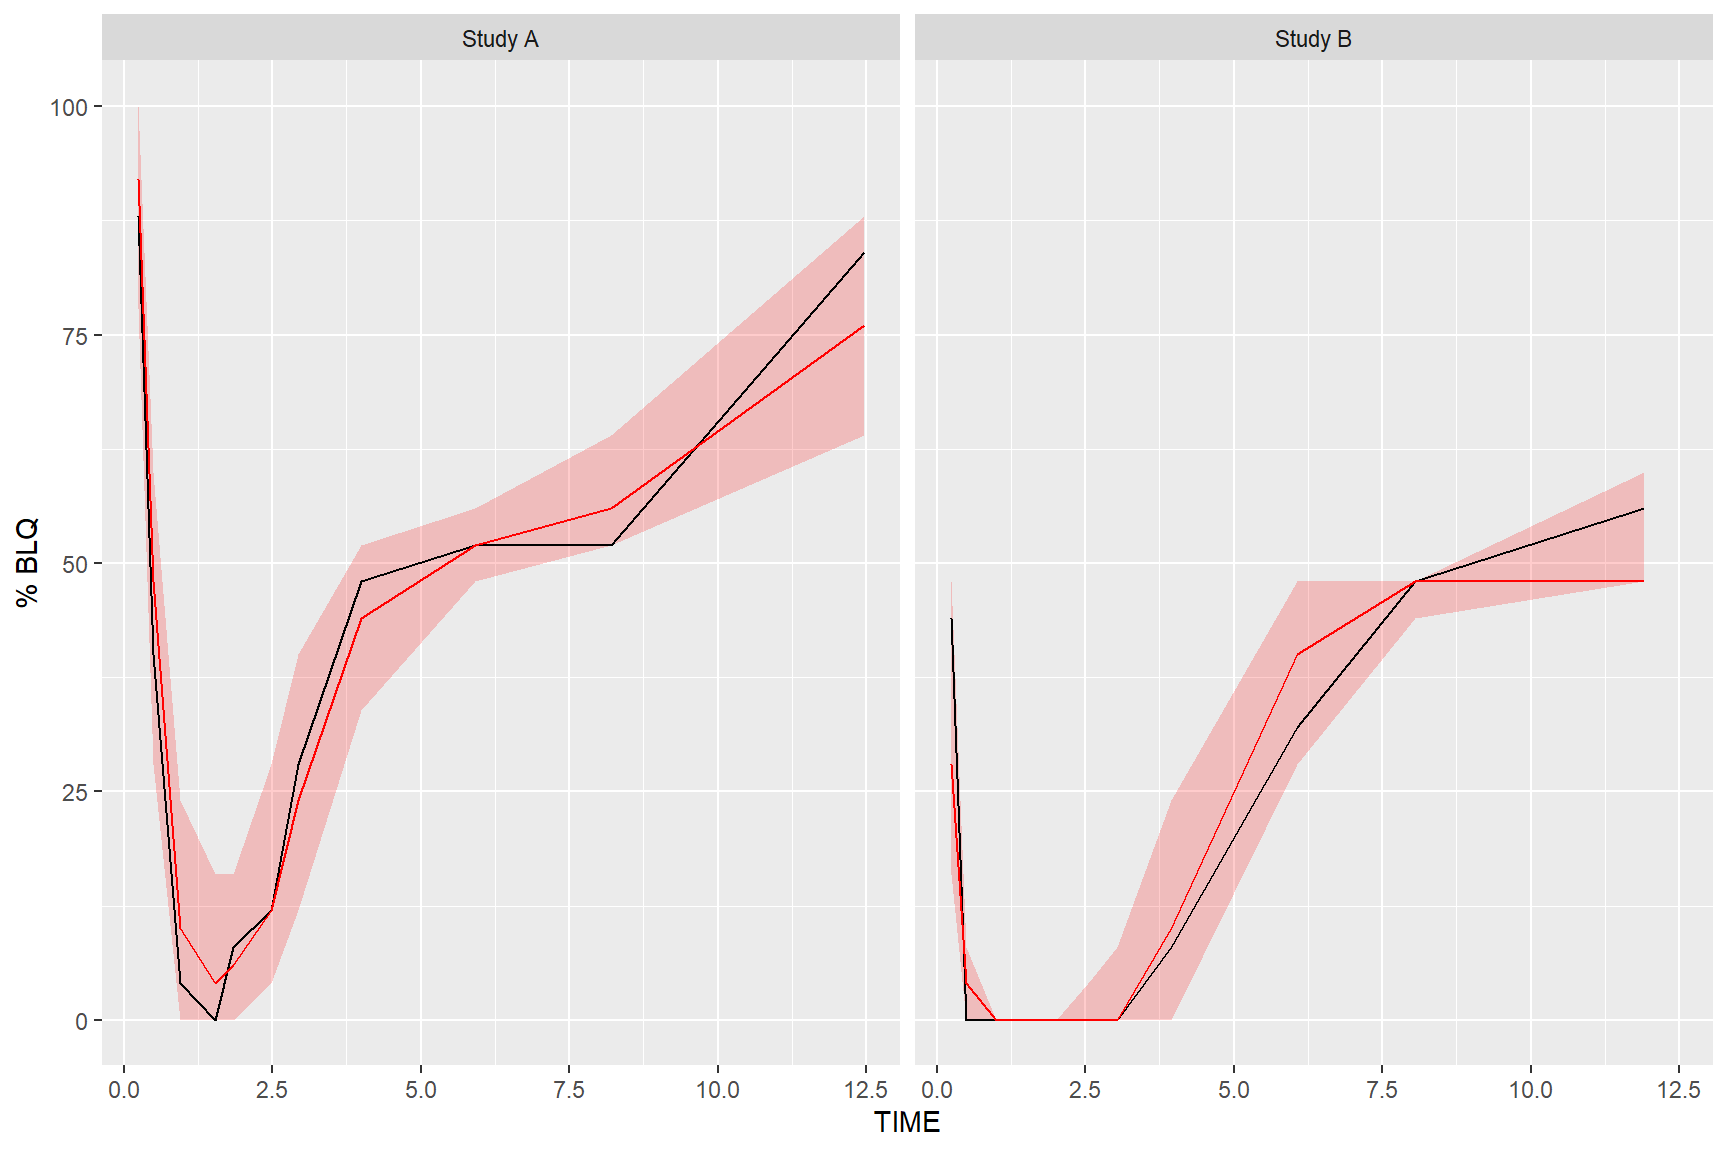
\includegraphics[width=640px]{tidyvpc_bookdown_files/figure-latex/unnamed-chunk-29-1}

\end{document}
